\documentclass[letterpaper,twocolumn,10pt]{z-article}

\usepackage{usenix2019_v3}

\newcommand{\sys}{SwitchCrypt}


% Shrink space between figs and text
% \setlength{\textfloatsep}{8pt plus 2pt minus 1pt}

% Shrink space between sections/subsections
% \usepackage{titlesec}
% \titlespacing\section{0pt}{8pt plus 2pt minus 1pt}{0pt plus 2pt minus 1pt}
% \titlespacing\subsection{0pt}{6pt plus 2pt minus 1pt}{0pt plus 2pt minus 1pt}
% \titlespacing\subsubsection{0pt}{6pt plus 2pt minus 1pt}{0pt plus 2pt minus 1pt}

%% Some recommended packages
\usepackage[normalem]{ulem}
\usepackage{booktabs}
\usepackage{pgfplotstable}
\usepackage{subcaption}
%\usepackage{natbib}
%\usepackage{epsfig}
%\usepackage[utf8x]{inputenc}
\usepackage{amsmath}
\let\Bbbk\relax
\usepackage{amssymb}
\usepackage{algorithm}
\usepackage{algorithmicx}
\usepackage[noend]{algpseudocode}
\usepackage{enumitem}      % adjust spacing in enums
%\usepackage{subfig}
%\usepackage{caption}
%\usepackage[hyphen]{url}

\usepackage{xspace}

%enumitem settings
\setlist{
  listparindent=\parindent,
  parsep=0pt,
}


%% Custom packages
% \usepackage{minted}  --- HSG haryadi disable it for a second
\usepackage{multirow}
\usepackage{rotating}
\usepackage{wrapfig}
\usepackage{tabu}
\usepackage{adjustbox}
\usepackage{pgfplots}
\usepackage{balance}
\usepackage{cleveref}
\usepackage{array}

% Fancy subsection references with cref
\crefformat{section}{\S#2#1#3} % see manual of cleveref, section 8.2.1
\crefformat{subsection}{\S#2#1#3}
\crefformat{subsubsection}{\S#2#1#3}

% Flexible table column specifications
\newcolumntype{C}[1]{>{\centering\arraybackslash}m{#1}}

%% Custom colors that are colorblind safe, print friendly, and photocopy safe
\definecolor{purpleDark}{RGB}{94, 60, 153}
\definecolor{purpleLight}{RGB}{178, 171, 210}
\definecolor{orangeDark}{RGB}{230, 97, 1}
\definecolor{orangeLight}{RGB}{253, 184, 99}

%% Custom fill patterns
\makeatletter
\pgfdeclarepatternformonly[\LineSpace]{custom north east lines}{\pgfqpoint{-1pt}{-1pt}}{\pgfqpoint{\LineSpace}{\LineSpace}}{\pgfqpoint{\LineSpace}{\LineSpace}}%
{
    \pgfsetcolor{\tikz@pattern@color}
    \pgfsetlinewidth{0.4pt}
    \pgfpathmoveto{\pgfqpoint{0pt}{0pt}}
    \pgfpathlineto{\pgfqpoint{\LineSpace + 0.1pt}{\LineSpace + 0.1pt}}
    \pgfusepath{stroke}
}

\pgfdeclarepatternformonly[\LineSpace]{custom north west lines}{\pgfqpoint{-1pt}{-1pt}}{\pgfqpoint{\LineSpace}{\LineSpace}}{\pgfqpoint{\LineSpace}{\LineSpace}}%
{
    \pgfsetcolor{\tikz@pattern@color}
    \pgfsetlinewidth{0.4pt}
    \pgfpathmoveto{\pgfqpoint{0pt}{\LineSpace}}
    \pgfpathlineto{\pgfqpoint{\LineSpace + 0.1pt}{-0.1pt}}
    \pgfusepath{stroke}
}
\makeatother

\newdimen\LineSpace
\tikzset{
    line space/.code={\LineSpace=#1},
    line space=3pt
}

%% Other custom colors
\definecolor{gray}{gray}{0.75}

% Ability to filter the values plotted from tables via `discard if not` key
\pgfplotsset{
    discard if symbol/.style 2 args={
        x filter/.append code={
            \edef\tempa{\thisrow{#1}}
            \edef\tempb{#2}
            \ifx\tempa\tempb
                \def\pgfmathresult{inf}
            \fi
        }
    }
}

\pgfplotsset{
    discard if symbol not/.style 2 args={
        x filter/.append code={
            \edef\tempa{\thisrow{#1}}
            \edef\tempb{#2}
            \ifx\tempa\tempb
            \else
                \def\pgfmathresult{inf}
            \fi
        }
    }
}

\pgfplotsset{
    discard if number/.style 2 args={
        x filter/.append code={
            \ifdim\thisrow{#1} pt=#2pt
                \def\pgfmathresult{inf}
            \fi
        }
    }
}

\pgfplotsset{
    discard if number not/.style 2 args={
        x filter/.append code={
            \ifdim\thisrow{#1} pt=#2pt
            \else
                \def\pgfmathresult{inf}
            \fi
        }
    }
}

%% Shortcuts
\newcommand{\ie}{\textit{i.e., }}
\newcommand{\eg}{\textit{e.g., }}
\newcommand{\CC}{C\nolinebreak\hspace{-.05em}\raisebox{.5ex}{\tiny\bf +}\nolinebreak\hspace{-.10em}\raisebox{.5ex}{\tiny\bf +}}

%% Units
\newcommand{\us}{\,$\mu$s}
\newcommand{\ms}{\,ms}
\newcommand{\KB}{\,KB}
\newcommand{\MB}{\,MB}
\newcommand{\GB}{\,GB}
\newcommand{\MHz}{\,MHz}
\newcommand{\GHz}{\,GHz}

%% Project name
\newcommand{\SystemURI}{https://github.com/ananonrepo2/\sys{}}%https://github.com/research/SwitchCrypt}

%% Reference parts of the paper
\newcommand{\figref}[1]{Fig.~\ref{fig:#1}}
\newcommand{\figsref}[2]{Figures~\ref{fig:#1} and~\ref{fig:#2}}
\newcommand{\figrref}[2]{Figures~\ref{fig:#1}--\ref{fig:#2}}
\newcommand{\secref}[1]{Section~\ref{sec:#1}}
\newcommand{\secsref}[2]{Sections~\ref{sec:#1} and~\ref{sec:#2}}
\newcommand{\eqnref}[1]{Eqn.~\ref{eqn:#1}}
\newcommand{\eqnsref}[2]{Equations~\ref{eqn:#1} and~\ref{eqn:#2}}
\newcommand{\eqnrref}[2]{Equations~\ref{eqn:#1}--\ref{eqn:#2}}
\newcommand{\insref}[1]{Instruction~\ref{ins:#1}}
\newcommand{\tblref}[1]{Table~\ref{tbl:#1}}
\newcommand{\appref}[1]{Appendix~\ref{app:#1}}
\newcommand{\algoref}[1]{Algorithm~\ref{algo:#1}}

\makeatletter
\newcommand\footnoteref[1]{\protected@xdef\@thefnmark{\ref{#1}}\@footnotemark}
\makeatother

%% Math
\newcommand{\argmin}{\arg\!\min}
\newcommand{\argmax}{\arg\!\max}
\newcommand{\minimize}{minimize}
\newcommand{\optimize}{optimize}
\newcommand{\ceil}[1]{\lceil #1 \rceil}
\newcommand{\floor}[1]{\lfloor #1 \rfloor}
\newcommand{\st}{s.t.}

%% Custom
\newcommand{\PUNT}[1]{}
\newcommand{\TODO}[1]{\textcolor{gray}{\textbf{\ [TODO:\ #1]\ }}}
\newcommand{\FIX}[1]{\textcolor{red}{\textbf{\ [FIX:\ #1]\ }}}
\newcommand{\hank}[1]{\textcolor{purple}{(Hank: #1)}}

%% For algorithms
\newcommand{\LineComment}[1]{\Statex \hfill\textit{#1}}

%% Configurations

\DeclareCaptionFormat{subfig}{\figurename~#1#2#3}
\DeclareCaptionSubType*{figure}
\captionsetup[subfigure]{format=subfig,labelsep=colon,labelformat=simple}

% Options for pgfplots
\pgfplotsset{compat=1.16,compat/show suggested version=false}
\usetikzlibrary{plotmarks}
\usetikzlibrary{calc}
\pgfplotsset{
    /pgfplots/bar  cycle  list/.style={/pgfplots/cycle  list={%
        {black,fill=black!30!white,mark=none},%
        {black,fill=red!30!white,mark=none},%
        {black,fill=green!30!white,mark=none},%
        {black,fill=yellow!30!white,mark=none},%
        {black,fill=brown!30!white,mark=none},%
    }},
}

% Begin of externalization
\usetikzlibrary{external}
\tikzexternalize[prefix=out/]
\tikzexternalize

% Ensure letter paper
\pdfpagewidth=8.5in
\pdfpageheight=11in

% Further configure pgfplots and tikz
\usetikzlibrary{patterns}
\usepgfplotslibrary{groupplots}
\pgfplotsset{
    every axis label/.append style={font=\small},
    tick label style={font=\small},
}

\pdfstringdefDisableCommands{
    \def\\{}
    \def\unskip{}
    \def\texttt#1{<#1>}
}

\graphicspath{{./figs/}{./data/}}

\pgfkeys{
    /pgf/number format/precision=1,
    /pgf/number format/fixed zerofill=true,
}

\pgfplotsset{
    nodes near coords greater equal only/.style={
        small value/.style={
            /tikz/coordinate,
        },
        every node near coord/.append style={
            check for small values/.code={
                \begingroup
                \pgfkeys{/pgf/fpu}
                \pgfmathparse{\pgfplotspointmeta<#1}
                \global\let\result=\pgfmathresult
                \endgroup
                \pgfmathfloatcreate{1}{1.0}{0}
                \let\ONE=\pgfmathresult
                \ifx\result\ONE
                    \pgfkeysalso{/pgfplots/small value}
                \fi
            },
            check for small values
        },
    },
}

\pgfplotsset{
    nodes near coords greater only/.style={
        small value/.style={
            /tikz/coordinate,
        },
        every node near coord/.append style={
            check for small values/.code={
                \begingroup
                \pgfkeys{/pgf/fpu}
                \pgfmathparse{\pgfplotspointmeta<=#1}
                \global\let\result=\pgfmathresult
                \endgroup
                \pgfmathfloatcreate{1}{1.0}{0}
                \let\ONE=\pgfmathresult
                \ifx\result\ONE
                    \pgfkeysalso{/pgfplots/small value}
                \fi
            },
            check for small values
        },
    },
}

% \author{Bernard Dickens III}
% \affiliation{
%   %\position{Position1}
%   %\department{Department1}              %% \department is recommended
%   \institution{University of Chicago}
%   % \streetaddress{5801 S Ellis Ave}
%   % \city{Chicago}
%   % \state{IL}
%   % \postcode{60637}
%   % \country{USA}
% }
% \email{bd3@cs.uchicago.edu}

% \author{Haryadi S. Gunawi}
% \affiliation{
%   %\position{Position1}
%   %\department{Department1}              %% \department is recommended
%   \institution{University of Chicago}
%   % \streetaddress{5801 S Ellis Ave}
%   % \city{Chicago}
%   % \state{IL}
%   % \postcode{60637}
%   % \country{USA}
% }
% \email{haryadi@cs.uchicago.edu}

% \author{David Cash}
% \affiliation{
%   %\position{Position1}
%   %\department{Department1}              %% \department is recommended
%   \institution{University of Chicago}
%   % \streetaddress{5801 S Ellis Ave}
%   % \city{Chicago}
%   % \state{IL}
%   % \postcode{60637}
%   % \country{USA}
% }
% \email{davidcash@cs.uchicago.edu}

% \author{Henry Hoffmann}
% \affiliation{
%   %\position{Position1}
%   %\department{Department1}              %% \department is recommended
%   \institution{University of Chicago}
%   % \streetaddress{5801 S Ellis Ave}
%   % \city{Chicago}
%   % \state{IL}
%   % \postcode{60637}
%   % \country{USA}
% }
% \email{hankhoffmann@cs.uchicago.edu}

\begin{document}


%% Title information

\def \mytitle {\sys: Kernel Support for Heterogeneous Full Drive Encryption}

% \title{\textsf{\textbf{\mytitle}}}

\title{\textsf{\mytitle}}

\author{Paper \#9}

\date{}

\maketitle


%% Abstract
\begin{abstract}

We introduce \sys, a secure storage system that provides block level kernel
support for {\em heterogeneous Full Drive Encryption} (FDE). Recent work on Full
Drive Encryption shows that stream ciphers achieve significantly improved
performance over block ciphers while offering stronger security guarantees.
However, optimizing for performance conflicts with concerns like battery life
and security. \sys takes advantage of the vast configuration space of stream
ciphers to balance these concerns via {\em cipher switching}. Our key insight in
achieving low-overhead switching is to leverage the overwrite-averse,
append-mostly behavior of underlying solid-state storage to trade throughput for
reduced energy use and powerful security properties. We implement \sys on an ARM
big.LITTLE mobile processor and test its performance under the popular F2FS file
system. Our evaluation shows \sys's heterogeneous FDE enables secure, flexible,
high-performance FDE with low overhead.


\end{abstract}


%% It begins!

\section{Introduction} \label{sec:introduction}



% ========================================================  INTRO

% about: security in general
Security is a very important property of storage systems.  Decades of 
systems and storage research in this space have looked into security in the context of 
V \cite{v1, v2, v3}, 
W \cite{w1, w2, w3}, 
X \cite{x1, x2, x3}, 
Y \cite{y1, y2, y3}, 
Z \cite{z1, z2, z3}, 
and many more.
% HSG: cite as many papers here from top systems venues
% until your reference hits 60 or more


% about: FDE/AES is bad
For local storage, the state of the art for securing data at rest, such as
the contents of a laptop's SSD, is Full Drive Encryption (FDE).
Unfortunately, encryption introduces overhead that drastically impacts
system performance and energy consumption.  FDE implementations such as
dm-crypt~\cite{dmcrypt,DmC-Android} for Linux and BitLocker for
Windows~\cite{bitlocker} are considered the standard available solutions.
Behind these implementations is the slow AES \emph{block cipher}
(AES-XTS)~\cite{XTS, XTSComments, NISTXTS}.  In this regard, the story of
Google's Android OS is a good example. Android supported FDE with the
release of Android 3.0, yet it was not enabled by default until Android
6.0~\cite{android-M-mobile-motivation}. Two years prior, Google attempted
to roll out FDE by default on Android 5.0 but had to backtrack. In a
statement to Engadget, Google blamed ``'performance issues on some partner
devices' ... for the backtracking''~\cite{google-engadget}. At the same
time, AnandTech reported a ``62.9\% drop in random read performance, a
50.5\% drop in random write performance, and a staggering 80.7\% drop in
sequential read performance'' versus Android 5.0 unencrypted storage for
various workloads~\cite{android-M-mobile-motivation-2}.



% about: recent advancements
Fortunately, in the last two years, there have been major advancements in
the FDE technology that distances away from the slow block cipher
technology and successfully implements {\em stream} chipers such as
ChaCha20 to full device encryption.  Recent works---such as Google's HBSH
(hash, block cipher, stream cipher, hash) \cite{hbsh-citation???},
Adiantum~\cite{Adiantum}, and StrongBox \cite{StrongBox}---brings stream
cipher based FDE to devices that do not or cannot support hardware
accelerated AES.  A key to efficiency adopt stream chiper into the storage
layer is to pair it with a log-structured file system such as F2FS
on flash devices (because \hsg{explain in one sentence}).


% about: the need flexibility
These advancements open up a new opportunity that: {\em can a file/storage
  system support multiple or flexible switching of full drive ecnryption?}
We postulate that such a feature is really needed but today we find {\em
  no} operating systems that can support such a feature.  To motivate this
feature, let's think about this one scenario: local files in a user's
mobile phone are ``forced'' to use encryption \encA because it is one of
the highest secured encryption that is safe for backing up the local files
to the cloud.  However when the mobile phone runs out of battery and is
doing a lot of I/Os, the heavy encryption will drain the battery down.
The user might wish a low battery mode where the data being accessed is
convered into a less powerful encryption momentarily.


% ======================================================== OUR SOLUTION


% about: the system and the benefits
We present \sys, to the best of our knowledge, the {\em first} kernel
support (at the block level) that provides file systems with flexible
switching of full drive encryption.  As FDE's impact on drive performance
and energy efficiency depends on a multitude of choices, different ciphers
expose different performance and energy efficiency characteristics.  \sys
allows cipher choice to be be viewed as a key configuration parameter, as
opposed to a static choice at format or boot time.  \sys allows
``encryption'' to adapt to changes that arise while the system is running,
including changes in resource availability, runtime environment, desired
security properties, and respecting changing OS energy budgets.  \sys
allows users to perform cipher switching in space and time (\eg, more
secure files and temporal switching).  \sys allows the software system to
navigate the tradeoff space made by balancing competing security and
latency requirements.  \hsg{This is where we list all the benefits; try
  not to be redundant} To achieve all these benefits, \sys comes with
three important elements, representing the three main contributions of the
paper.


% about: switching strategies
First, we introduce \sysA, a kernel configuration that exposes three types of
switching models {\em forward}, {\em selective} and {\em mirrored}, to to
``re-cipher'' storage units dynamically, allowing us to tradeoff different
performance and security properties of various configurations at runtime.
These switching models define what the I/O layer should do upon the
ongoing read/write I/Os during the switching.  These three switching
models are motivated from real case studies.  For examples, forward
switching is motivated from the battery case study above; selective
switching is motivated from cases where users desire to have certain files
(\eg, legal documents) much more secure than the others; and mirrored
switching is motivated for server-side cases that would like to perform
``encryption upgrade'' without zero downtime.

% about: crypts
Second, to supports the switching models above, we implement \sysB, a
block-level module that contains encryption implementations (``crypts'')
that have been restructured to support switching.  Prior works mainly
implement one cipher choice and the implementation is very much integrated
with the file/block layer \cite{StrongBox, any-other-works-like-this?}.
The key challenge to support multiple ciphers is that different chipers
take different inputs and produce different type of outputs.  For
examples, \encA requires nonce input, \encB config(??\xxx) and \encC
sector info and \encC outputs streams while the others output \xxx.  Thus,
we introduce a novel design substantively expanding prior FDE work by
wholly decoupling cipher implementations from the encryption process.  In
\sysB, we wrote hooks that manages the required input values and the
output format of different ciphers.


% about: tradeoffs
Finally, we initiate \sysC, a scheme that attempts to {\em quantify} the
tradeoffs in the the rich configuration space of stream ciphers.  Using
this scheme, we define a tradeoff space of cipher configurations over
competing concerns: total energy use, desirable security properties, read
and write performance (latency), total writable space on the drive, and
how quickly the contents of the drive can converge to a single encryption
configuration.  \sysC helps users in understanding their cipher choices as
they come with a variety of performance, energy efficiency, and security
properties in the FDE context.


% about: evaluation 
We performed a comprehensive evaluation in several ways.
%
First, we show that \sys successfully supports a wide variety of ciphers;
specifically we have integrated {\em \numCiphers ciphers} and a total of
{\em \numConfigs cipher configurations} into \sys in \locTotal as a kernel
block module (will be open-sourced), and can act as an off-the-shelf
replacement for dm-crypt.  The ciphers are ChaCha8 and
ChaCha12~\cite{ChaCha20}, Freestyle~\cite{Freestyle}),
SalsaX~\cite{SalsaX}, AES in counter mode (AES-CTR)~\cite{AESCTR},
Rabbit~\cite{Rabbit}, Sosemanuk~\cite{Sosemanuk}, \xxx.
%
Second, we showcase the benefits of \sys with experiments illustrating
three real-world case studies (battery low case, file-level protections,
and no downtime) and show the performance/energy tradeoffs.
%
Finally, we perform several benchmarking to show the performance and \xxx
of the individual ciphers and the switching overhead of the three
switching models we provide \hsg{???}.



\section{Background and Motivation} \label{sec:motivation}


We provide some case studies that motivate our work and background
materials about implementation of stream cipher on log-structured file
systems.





\mysub{File encryption reacting to battery saver}



% =======================================================
\subsection{The Static FDE Problem}

The major issue with full drive encryption (FDE) is its static nature;
users must commit one FDE configuration without much flexibility.  Let us
suppose we have an ARM-based ultra-low-voltage netbook provided to us by
our employer who requires that the drive is fully encrypted at all times
and is constantly backed up to an offsite system.  Given that the FDE
industry standard is AES-XTS, we initialize our drive with it.  Here,
three primary concerns present themselves: performance, vulnerability and
inflexibility.

First, it is well known that AES-XTS adds significant latency and power
overhead to I/O operations, especially on mobile and battery-constrained
devices~\cite{google-engadget, android-M-mobile-motivation,
  android-M-mobile-motivation-2}.  As this scenario requires the drive
encrypted at all times, we must accept this hit to performance and battery
life.  Worse, if our device does not support hardware accelerated AES
(which is hardly ubiquitous) performance can be degraded even further; I/O
latency can be as high as 3--5x~\cite{StrongBox}.

% As myriad devices do not support it cannot simply be ignored, hence
% Google's investment in Adiantum---an FDE solution for ``the next billion
% users'' of low-cost devices without support for hardware accelerated
% AES~\cite{Adiantum}.

Second, AES-XTS is designed to mitigate threats to drive data ``at rest,''
which assumes an attacker cannot access snapshots of our encrypted data
nor manipulate our data without those manipulations being immediately
obvious to us. However, access to multiple snapshots of a drive's
AES-XTS-encrypted contents presents a vulnerability---an attacker can
passively glean information about the plaintext over time by contrasting
those snapshots, leading to confidentiality violations in some
situations~\cite{XEX, XTS}.  In this case, we might want to employ a
strong encryption solution such as stream ciphers, but they are known to
perform worst in many file systems.

Third, our system is battery constrained, placing a cap on our energy
budget that can change at any moment as we transition from line power to
battery power and back.  Our system should respond to these changing
requirements without violating any other concerns.



% =======================================================
\subsection{Recent Advancements}

In this paper we categorize two types of FDE: {\em block} and {\em stream} chipers.
Block chipers were a defacto solution for storage while stream chipers
were prevalent in networking \hsg{true??}.  Their main differences are
\hsg{fill here, 1 or 2 sentences}.
% ............
There have been major advancements in the FDE
technology that distances away from the slow block cipher technology and
successfully implements stream chipers full device encryption
\cite{Adiantum, StrongBox} even without hardware
accelerated encryption.  


There are two technological shifts that enable this confidential,
high-performance storage with stream ciphers.  First, devices today
commonly employ solid-state storage with Flash Translation Layers (FTL),
which operate similarly to Log-structured File Systems (LFS) \cite{21, 22,
  27-fromStrongBox}.  The no inplace update nature of FTL or LFS-like
storage allows the overwrite-heavy stream chipers to be efficiently
implemented (\eg, ChaCha with F2FS or LogFS performs \xxx times better
than with ext4 \cite{StrongBox}).  Second, mobile devices now support
trusted hardware, such as Trusted Execution Environments (TEE) \cite{24,
  29-fromStrongBox} and secure storage areas \cite{10-fromStrongBox} which
means the drive encryption module has access to persistent, monotonically
increasing counters that can be used to prevent rollback attacks when
overwrites do occur.


% =======================================================
\subsection{No One-Size-Fits-All Case Studies}

As the recent advancements show that many different ciphers can be
implemented in efficient manner, this opens up an opportunity for the
storage layer to support a wide variety of encryption technologies.
Clearly, many case studies show that there is no one-size-fits-all
encryption, and some flexibility is demanded.  Below we present three
real-wrold case studies.

{\em Battery-life saver.}  In the example above, in certain situations,
the user might want to prioritize reducing the total energy use.  For
example, while in battery low mode, the kernel now switches to a more
energy-efficient encryption and pauses the offline cloud backup
moementarily.  Users might be willing to accept this tradeoff and violate
the ``backup at all time'' rule, knowing that within a few hours the user
will have access to power (no difference from internet connection
problem).  This case study is pervasive
\cite{hackernews-???, many-more??}.


{\em Cipher upgrade without downtime.}  From mobile devices, we now turn
to server-side storage that often require encryption upgrade
\cite{some-citations}.  A server provider might decide to completely
upgrade from a encryption technology that has been broken into a stronger
encryption technology.  Ideally during the switch, the server still can
continuously serves users without any downtime.  However, without
kernel-level support, the server provider must write an application level
software that performs the whole switching operation and manually
redirects users to the appropriate files.



{\em Select files.}  Learning from the wireless literature, it is
advocated that certain files that traverse the Internet or wireless
connection in particular, should be encryption with a more secure way.
Example of those files include government documents
\cite{citation-to-this-example}, credit card information \cite{a}, \xxx
\cite{a, b, c}.


%
\if 0
\section{SwitchCrypt Design} \label{sec:design}

\subsection{SwitchCrypt Overview} \label{subsec:overview}

\begin{figure}[ht]
   \centering
   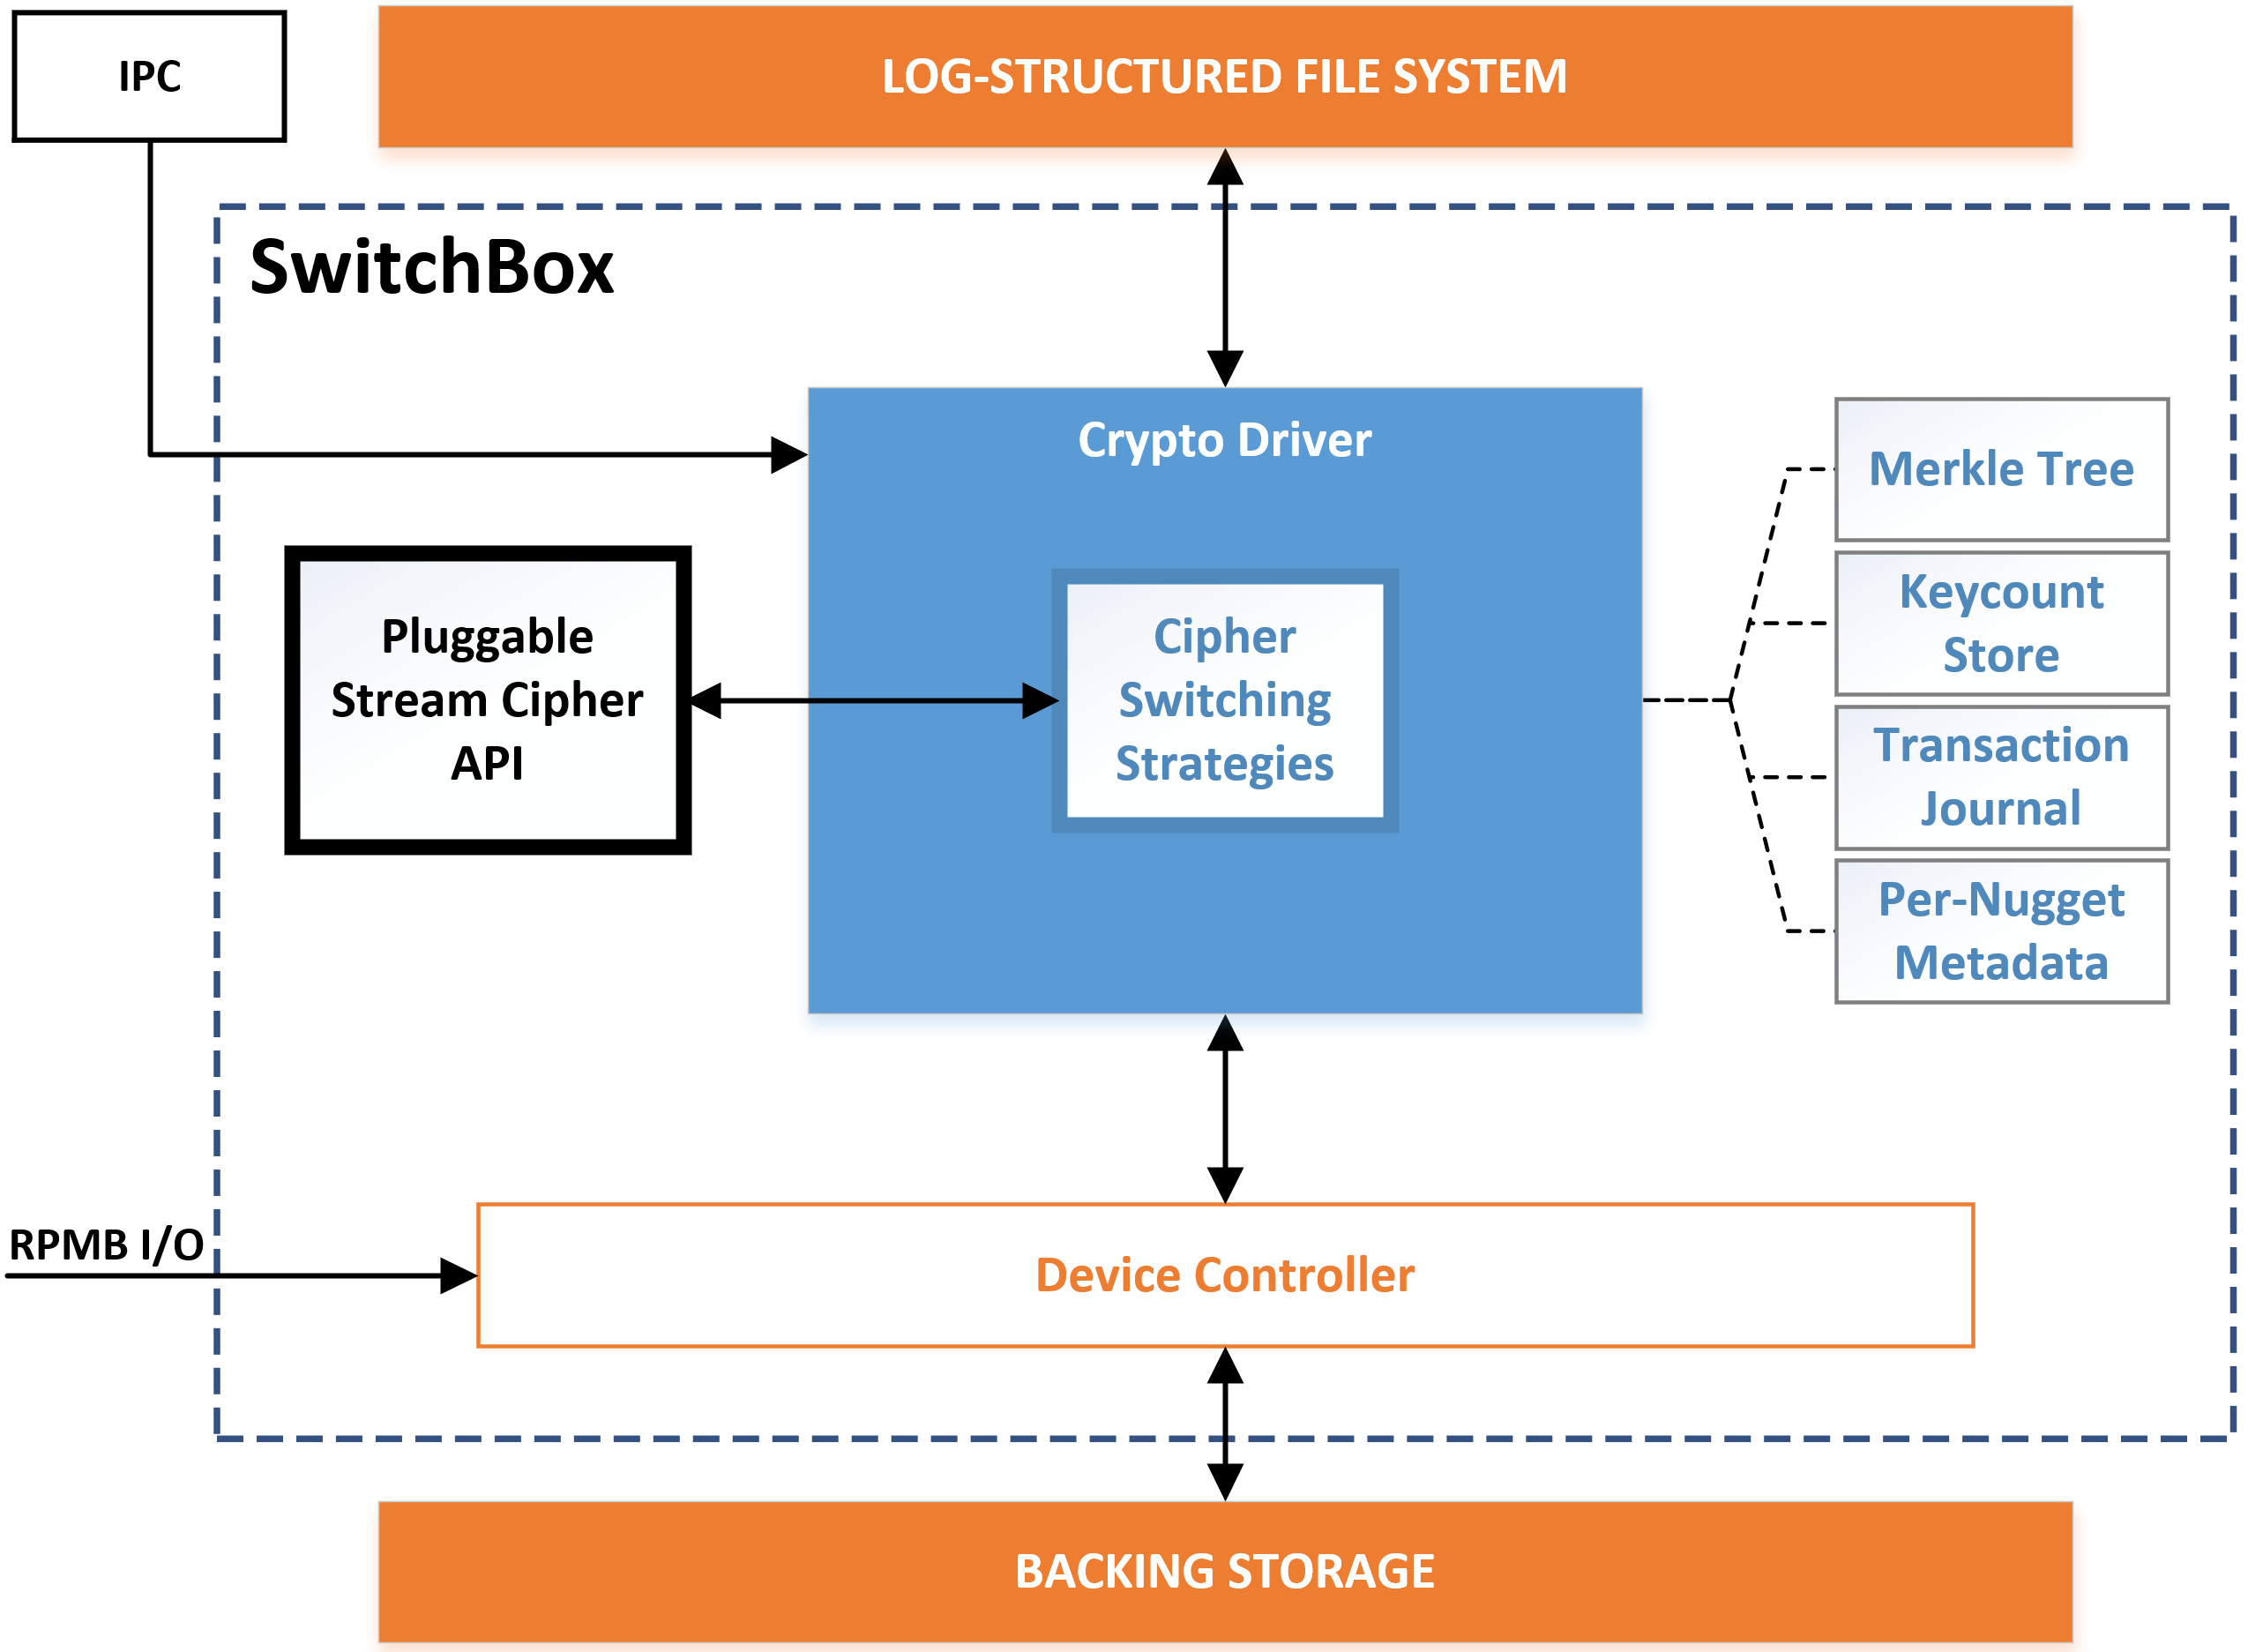
\includegraphics[width=\linewidth]{overview.png}
   \caption{Overview of the SwitchCrypt construction.} \label{fig:overview}
\end{figure}

SwitchCrypt consists of a \emph{Generic Stream Cipher Interface} and
\emph{Cryptographic Driver}; SwitchCrypt sits between a Log-structured File
System (LFS) on the OS, and the underlying drive (backing storage) and device
controller (e.g. Flash Translation Layer). This is illustrated in
\figref{overview}, which provides an overview of the SwitchCrypt system design.

\begin{figure}[t]
   \centering
   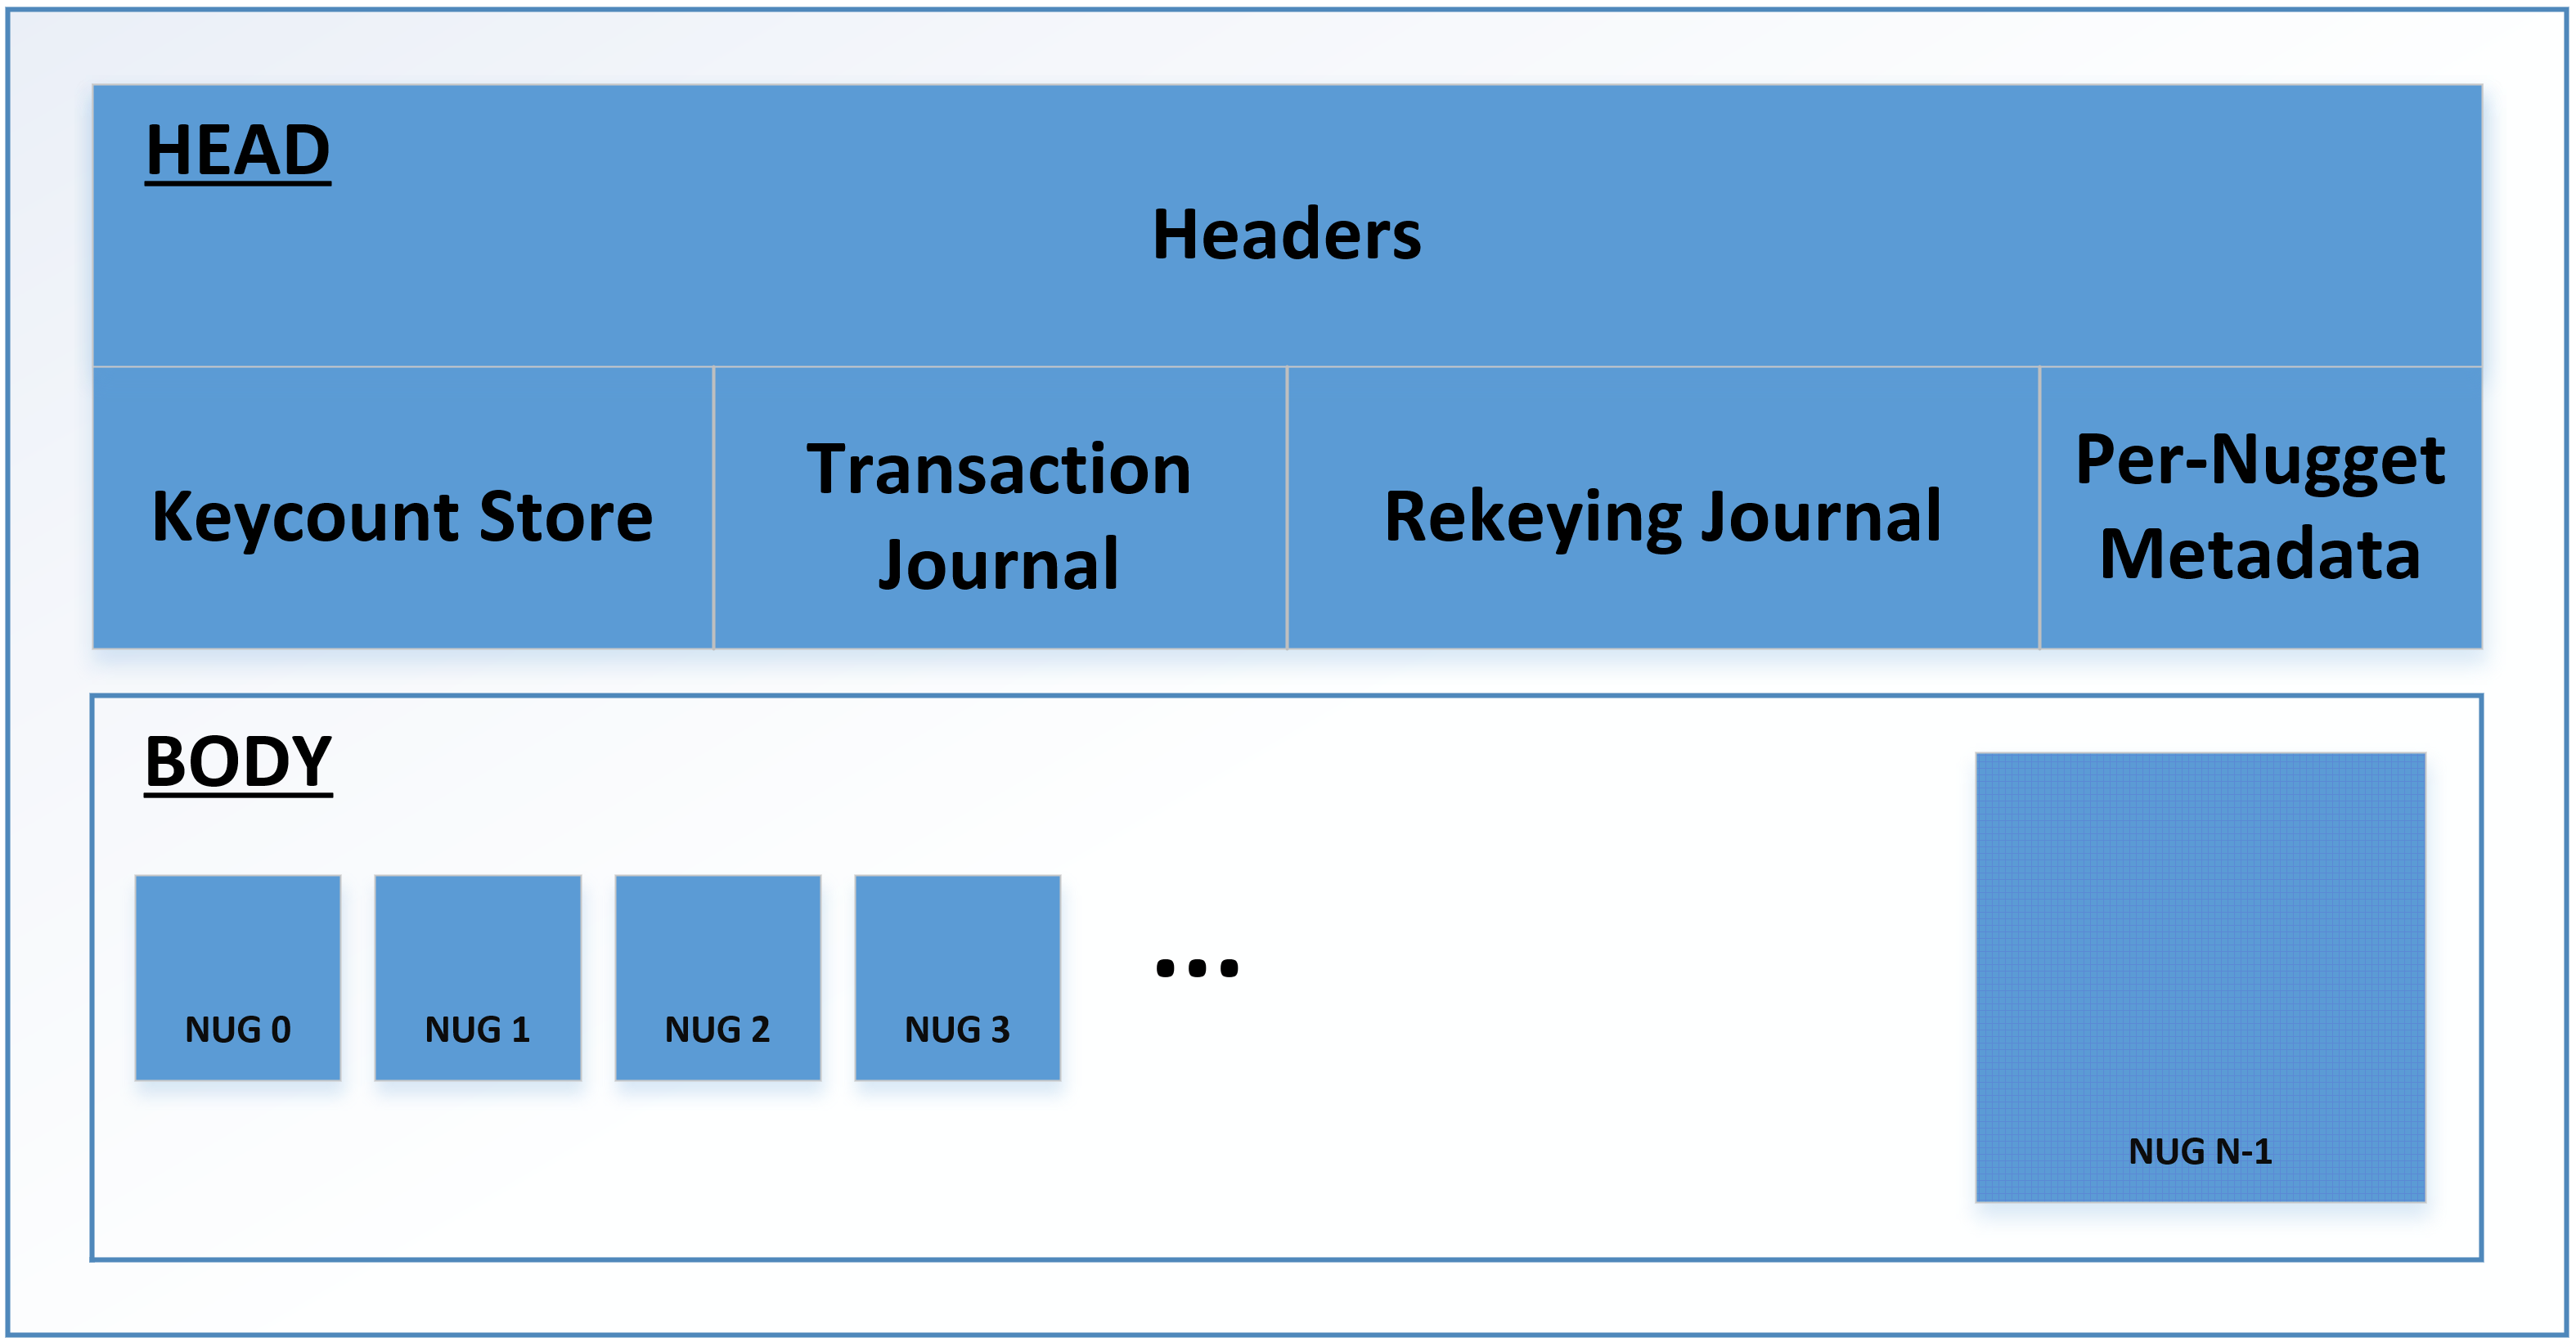
\includegraphics[width=\linewidth]{backstore.png}
   \caption{Layout of SwitchCrypt's drive layout.} \label{fig:backstore}
\end{figure}

The drive itself is divided into a \emph{HEAD} section and \emph{BODY} section
upon initialization, illustrated in \figref{backstore}. The HEAD consists of
metadata headers written during initialization~\cite{StrongBox} along with the
\emph{Keycount Store}, \emph{Transaction Journal}, \emph{Rekeying Journal}, and
\emph{Per-Nugget Metadata}, each drive-backed. These components are used by the
\emph{Cryptographic Driver} together with the \emph{Cipher Switching Strategy}
implementations to enable efficient per-unit cipher switching.

The BODY consists of a series independent same-size logical units called
\emph{nuggets}. A nugget consists of one or more contiguous physical drive
blocks. Each nugget is coupled with metadata in the HEAD indicating which cipher
was used to encrypt the nugget along with any additional ciphertext output; the
latter allows us to treat any non-length-preserving ciphers as if they were
length-preserving. SwitchCrypt uses the Keycount Store and Transaction Journal
components along with our nugget layout to 1) track, detect, and handle
overwrites, 2) limit the maximum length of any plaintext input to ciphers, thus
amortizing the overhead incurred during encryption, and 3) independently and
efficiently switch the cipher used to encrypt individual nuggets.

Dickens et al. showed how to make nugget-based drive organization secure using a
single stream cipher, ChaCha20, to handle overwrites, prevent rollback attacks,
and limit plaintext length~\cite{StrongBox}. However, they did not envision the
utility in trading off between concerns at the filesystem or device-mapper
level, dynamic cipher switching, or protecting against attacks on data ``in
motion;'' the remainder of this section details the novel components that enable
this functionality. Specifically: how we quantify the properties traded off
between configurations (\cref{subsec:quantify}), the Generic Stream Cipher
Interface and Per-Nugget Metadata components (\cref{subsec:interface}) which
decouple cipher implementations from the encryption process, and our Cipher
Switching Strategy implementations (\cref{subsec:strategies}) used to
efficiently encrypt nuggets with different ciphers.

\subsection{Quantifying Cipher Security Properties} \label{subsec:quantify}

To reason about when to trade off between the ciphers evaluated in this work, we
must have a way to compare ciphers' utility in the context of SwitchCrypt FDE.
However, different ciphers have a wide range of security properties, performance
profiles, and output characteristics. To address this need, we propose a novel
evaluation framework (see: \tblref{security-quant}). Our framework classifies
stream ciphers according to three quantitative features: relative round count,
ciphertext randomization, and ciphertext expansion. Taken together, these
features reveal a rich tradeoff space of cipher configurations optimizing for
different combinations of concerns.

\begin{table}[ht]
   \begin{tabular}{@{}ccccc@{}}
   \toprule
   \textbf{Cipher} & \textbf{Rounds} & \textbf{Randomization} &
   \textbf{Expansion} \\
   \midrule
   ChaCha8         & 0           & 0           & 1           \\
   ChaCha12        & 0.5         & 0           & 1           \\
   ChaCha20        & 1           & 0           & 1           \\
   Salsa8          & 0           & 0           & 1           \\
   Salsa12         & 0.5         & 0           & 1           \\
   Salsa20         & 1           & 0           & 1           \\
   HC128           & 0           & 0           & 1           \\
   HC256           & 1           & 0           & 1           \\
   Freestyle (F)   & 0           & 2           & 0           \\
   Freestyle (B)   & 0.5         & 2.5         & 0           \\
   Freestyle (S)   & 1           & 3           & 0           \\
\end{tabular}
   \caption{Our framework for classifying stream ciphers according to three
   ideal features: relative round count, ciphertext randomization, and
   ciphertext expansion.}
   \label{tbl:security-quant}
 \end{table}

\subsubsection{Relative Rounds (Rounds)}

The ciphers we examine in this paper are all constructed around the notion of
\emph{rounds}, where a higher number of rounds (and possibly longer key) is
positively correlated with a higher resistance to brute force given no fatal
related-key or other attacks~\cite{ChaCha-Cryptanalysis}. Hence, this feature
represents how many rounds a cipher executes relative to other implementations
of the same algorithm. For instance: ChaCha8 is a reduced-round version of
ChaCha12, which is a reduced-round version of ChaCha20, all using the ChaCha
algorithm~\cite{ChaCha20,ChaCha-Cryptanalysis}.

We limit our analysis to groups of three implementations, each using a different
number of rounds. In the case of HC-128 and HC-256, we limit our analysis to a
group of two implementations. Scores range from 0 (least number of rounds
considered) to 1 (greatest number of rounds considered).

\subsubsection{Ciphertext Randomization (Randomization)}

A cipher with ciphertext randomization generates different ciphertexts
non-deterministically given the same key, nonce, and plaintext. This makes it
much more difficult to execute chosen-ciphertext attacks (CCA), key
re-installation attacks, XOR-based cryptanalysis and other comparison attacks,
and other confidentiality-violating schemes where the ciphertext is in full
control of the adversary ~\cite{Freestyle}. This property is useful in cases
where we cannot prevent the same key, nonce, and plaintext from being reused,
such as with data ``in motion'' (see the motivational example earlier in this
work). Ciphers without this property---such as ChaCha20 on which prior work is
based---are trivially broken when key-nonce-plaintext 3-tuples are reused. In
StrongBox, this is referred to as an ``overwrite condition'' or simply
``overwrite''~\cite{StrongBox}.

Though there are many ways to achieve ciphertext randomization, the ciphers
included in our analysis implement it using a random number of rounds for each
block of the message where the exact number of rounds are unknown to the
receiver a priori~\cite{Freestyle}. In determining the minimum and maximum
number of rounds used per block in this non-deterministic mode of operation, we
can customize the computational burden an attacker must bear by choosing lower
or higher minimums and maximums. Hence, this is not a binary feature; scores
range from 0 (no ciphertext randomization) to 1 (lowest minimum and maximum
rounds per block) to 3 (highest minimum and maximum rounds per block).

\subsubsection{Ciphertext Expansion (Expansion)}

A cipher that exhibits ciphertext expansion is non-length-preserving: it outputs
more or less ciphertext than was originally input as plaintext. This can cause
major problems in the FDE context. For instance, cryptosystems that rely on
AES-XTS (e.g. Linux's dm-crypt, Microsoft's BitLocker, Apple's FileVault) or
ChaCha (e.g. StrongBox, Google's Adiantum) have storage layouts that hold
length-preserving output as an invariant, making ciphers that do not exhibit
this property incompatible with their implementations; yet, ciphertext expansion
is often (but not always) a necessary side-effect of ciphertext randomization.

The ciphers included in our analysis that exhibit ciphertext expansion have an
overhead of around 1.56\% per plaintext message block~\cite{Freestyle}. Even a
single byte of additional ciphertext vs plaintext would make a cipher
inappropriate for use with prior work. Hence, this is a binary feature in that a
cipher either outputs ciphertext of the same length as its plaintext input or it
does not. A cipher scores either a 0 if it \emph{is not} length-preserving in
this way or a 1 if the ciphertext is always the same length as the plaintext.

\subsection{Generic Stream Cipher Interface} \label{subsec:interface}

One of the goals of SwitchCrypt is that we might use any stream cipher
regardless of its implementation details. Yet this is entirely non-trivial.
There are many cipher implementations that we might use with SwitchCrypt, each
with unique input requirements and output considerations. For instance, Salsa
and Chacha implementations require a certain IV and key size and handle
plaintext input through successive invocations of a single state update
function~\cite{Floodyberry}. Using OpenSSL's AES implementation in CTR mode
requires manually tracking the counter state and individual ciphertext blocks
are retrieved though corresponding function invocations~\cite{OpenSSL}.
Freestyle's reference implementation requires we calculate the extra space
necessary per nugget (due to ciphertext expansion) along with
configuration-dependent minimum and maximum rounds-per-block, hash interval, and
pepper bits~\cite{Freestyle}. HC-128 and other ciphers have similarly disparate
requirements.

Unlike prior work, SwitchCrypt must be able to encrypt and decrypt arbitrary
nuggets \emph{with any of these ciphers} at any moment with low overhead and
without tight coupling to any specific implementation detail. Hence, there is a
need for an interface that completely decouples cipher implementations from the
encryption/decryption process. Our novel cipher interface allows any stream
cipher to be integrated into SwitchCrypt without modifications to third-party
code, enabling normally incompatible ciphers to encrypt and decrypt arbitrary
nuggets. The ability for disparate cipher implementations to co-exist forms the
foundation for SwitchCrypt's ability to switch the system between different
cipher configurations in our tradeoff space efficiently and effectively.

To facilitate this, the Generic Stream Cipher Interface presents the
cryptographic driver with a single unified encryption/decryption model.
SwitchCrypt receives I/O requests from the operating system at the block device
level like any other device-mapper. These requests come in the form of either
reads or writes. When a read request is received, the OS hands SwitchCrypt an
offset and a length and expects a response with plaintext of that specific
length starting at that specific offset taken from the beginning of storage
(i.e. the BODY section; see \figref{backstore}). When a write request is
received, the OS hands SwitchCrypt an offset, a length, and a buffer of
plaintext and expects that plaintext to be encrypted and committed to storage
such that the plaintext is later retrievable given that same offset and length
in a future read request. These requests can either be handled together by a
single function or handled individually as distinct read and write operations,
each with different tradeoffs.

\begin{enumerate}
   \item \textbf{\texttt{xor\_interface}}\\\texttt{xor\_interface} executes
   independently of SwitchCrypt internals and treats encryption and decryption
   as the same operation. Implementations receive an integer offset $F$, an
   integer length $L$, a key buffer $K$ corresponding to the current nugget, and
   an empty $L$-length XOR buffer. SwitchCrypt expects the XOR buffer to be
   populated with $L$ bytes of keystream output from some stream cipher seeked
   to offset $F$ with respect to key $K$. The length of the key buffer will
   always be exactly what the cipher implementation expects, alleviating the
   burden of key management; similarly, the XOR buffer will be XOR-ed with the
   appropriate portion of nugget contents automatically, alleviating the burden
   of drive access and other tedious calculations. \\
   \item \textbf{\texttt{read\_interface}} and
   \textbf{\texttt{write\_interface}}\\
   Unlike \texttt{xor\_interface}, encryption and decryption are distinct
   concerns at this abstraction level. \\\texttt{read\_interface} handles
   decryption during reads. \\\texttt{write\_interface} handles encryption
   during writes. Implementations receive full access to SwitchCrypt internals,
   giving wrapper code complete control over the encryption and decryption
   process and allowing implementers to bypass parts of the nugget-based drive
   layout abstraction (i.e. BODY) if necessary. This comes at the cost of 1)
   significantly increased code complexity, as the implementer must perform
   certain I/O manually, distinguish between independent nuggets on the drive,
   determine what to encrypt or decrypt at what offset and when, when to commit
   which metadata and where and 2) potential performance implications, since
   SwitchCrypt must account for not having absolute control over its internal
   data structures during function invocation. For a cipher like Freestyle,
   configurations with lower minimum and maximum rounds per block may see a
   performance improvement here, while configurations with higher minimum and
   maximum rounds per block may see reduced performance.
\end{enumerate}

\subsection{Cipher Switching Strategies} \label{subsec:strategies}

The Generic Stream Cipher Interface allows many differently ciphered nuggets to
co-exist on the same drive. However, at any moment, there is only a single
\emph{active cipher configuration} (henceforth \emph{active configuration}). The
active configuration is used to encrypt nugget contents. When a cipher switch is
triggered, a different configuration becomes the active configuration. At this
point, SwitchCrypt must determine \emph{when} to re-cipher a nugget and
\emph{where} to store the output on the drive. ``Re-ciphering'' here means using
an inactive configuration to decrypt a nugget's contents and using the active
configuration to re-cipher it. Depending on the use case, it may make the most
sense to re-cipher a nugget immediately, or eventually, or to maintain several
areas of differently-ciphered nuggets concurrently.

A naive approach would switch every nugget in BODY to the active configuration
immediately, but the latency and energy cost would be unacceptable. Hence, a
more strategic approach is necessary. We satisfy this need with our \emph{cipher
switching strategies}. These novel strategies allow for nuggets to be
re-ciphered in a variety of cases with minimal impact on performance and battery
life and without compromising security. This is thanks to the nugget-based drive
layout, which limits the churn of cipher switching operations to relatively
small regions of ciphertext on the drive.

Determining \emph{when} to target a nugget for re-ciphering we call
\emph{temporal switching}, for which we propose the \emph{Forward} switching
strategy. Determining \emph{where}---in which storage region and across which
nuggets---to output ciphertext we call \emph{spatial switching}, for which we
propose the \emph{Mirrored} and \emph{Selective} switching strategies.

\textbf{Forward Switching Strategy.} When a nugget is encountered during I/O
that was encrypted using something other than the active configuration, the
Forward strategy dictates that this nugget be re-ciphered immediately. If a
particular nugget encrypted with an inactive configuration is never encountered
during I/O, it is never re-ciphered and remains on the drive in its original
state. In this way, the Forward strategy represents a form of temporal cipher
switching.

Rather than re-cipher the entire drive every time the active configuration
changes, this strategy limits the performance impact of cipher switching to
individual nuggets. The expense of re-ciphering is paid only once, after which
the nugget is accessed normally during I/O until the active configuration is
switched again.

\PUNT{There are several forms the Forward strategy might take. The default and
most intuitive is \emph{0-forward}, in which SwitchCrypt immediately transitions
individual nuggets encountered during I/O to the active configuration if they
are not using it. Over time, if various I/O operations end up touching every
nugget in the drive, the encrypted contents of every nugget will become
decryptable with the currently active configuration.

The Forward strategy might also take the form of \emph{N-forward}, where
SwitchCrypt attempts to take advantage of spatial sequential locality to
transition whole sets of nuggets into the active configuration. We can trivially
expand the forward strategy to encompass the entire drive by selecting $N$ equal
to the total number of nuggets managed by SwitchCrypt. This would have the
overhead of re-ciphering large swaths of the drive upon every I/O operation
where a nugget encrypted with the inactive configuration is encountered. Of
course, this has the same dire implications for performance as simply
re-initializing the entire system or encrypted container with the new cipher.}

\textbf{Selective Switching Strategy.} When SwitchCrypt is initialized with the
Selective strategy, the drive is partitioned into $C$ regions where $C$
represents the total number of available ciphers in the system; each regions'
nuggets are encrypted by each of the $C$ ciphers respectively. For instance,
were SwitchCrypt initialized using two ciphers ($C = 2$), the drive would be
partitioned in half; all nuggets in the first region would be encrypted with the
first cipher while all nuggets in the second would be encrypted with the other.


When using this strategy, the active cipher determines which partition we
``select'' for I/O operations. Hence, unlike the Forward strategy, which
schedules individual nuggets to be re-ciphered at some point in time after the
active configuration is switched, the Selective strategy allows the wider system
to indicate \emph{where} on the drive a read or write operation should occur. In
this way, the Selective strategy represents a form of spatial cipher switching
where different regions of the drive can store differently-ciphered nuggets
independently and concurrently. A user could take advantage of this to, for
instance, set up regions with different security properties and performance
characteristics, managing them as distinct virtual drives or transparently
reading/writing bytes to different security regions on the same drive.

\textbf{Mirrored Switching Strategy.} Similar to the Selective strategy, when
SwitchCrypt is initialized with the Mirrored strategy, the drive is partitioned
into $C$ regions where $C$ represents the total number of available ciphers in
the system; each regions' nuggets are encrypted by each of the $C$ ciphers
respectively.

However, unlike the Selective strategy, all write operations that hit one region
are mirrored into the other regions immediately, so all regions of the drive
will always be in a consistent state and always share the same data. The active
configuration determines \emph{where} a read operation should occur. In this
way, the Mirrored strategy represents a form of spatial cipher switching because
we're switching which configuration we're using to read in data. A user could
take advantage of this along with SSD Instant Secure Erase~\cite{ISE1,ISE2,ISE3}
to delete other regions, thus quickly and securely converging the drive to a
single configuration without losing any data or suffering the egregious
performance or battery penalty that comes with re-ciphering every nugget.

\subsubsection{Comparing Cipher Switching Strategies}

\begin{table}[ht]
   \begin{tabular}{@{}|c|c|c|C{25mm}|@{}}
      \toprule
      \textbf{Strategy} & \textbf{Convergence} & \textbf{Waste} &
      \textbf{Performance} \\
      \midrule
      Forward   & Slower       & None & Faster reads and writes unless switching
      \\\hline
      Mirrored  & Nearly instant & High & Faster reads; slower writes \\
      \hline
      Selective & Slower       & High & Faster reads and writes  \\
      \hline
   \end{tabular}
   \caption{A summary comparison between the three cipher switching strategies.}
   \label{tbl:strategies-advantages}
\end{table}

\tblref{strategies-advantages} summarizes the higher level tradeoffs between the
three cipher switching strategies.

\textbf{Convergence.} Depending on the use case, the ability to quickly converge
the entire drive to a single cipher configuration without losing data is very
useful (see: \secref{usecases}). The near-instantaneous ``just forget the key''
nature of SSD Instant Secure Erase (ISE) implementations on modern
SSDs~\cite{ISE1,ISE2,ISE3} makes this a very fast process for the Mirrored
strategy. The Forward strategy is slow to converge compared to Mirrored since,
in the worse case, every nugget on the drive will require re-ciphering. The
Selective strategy is similarly slow to converge since entire regions of nuggets
must be moved and re-ciphered to prevent data loss; those regions could be
destroyed without moving data around using ISE too, which would be very fast,
but unlike Mirrored some data would be lost forever.

\textbf{Waste.} Unlike the other two strategies, using the Forward strategy does
not reduce the total usable space on the drive by the end-user, ciphertext
expansion notwithstanding. We refer to this as ``waste''. The Forward strategy
is not wasteful in this way because it allows differently-ciphered nuggets to
co-exist contiguously on the drive without special partitions. Since the
Mirrored and Selective strategies require partitioning the drive into some
number of regions---where the writeable size reported back to the OS is some
function of region size---there is a necessary reduction in usable space.

\textbf{Performance.} The Selective and Mirrored strategies can read data from
the drive with low overhead, reaching performance parity with prior work,
because they never have to deal with on-demand re-ciphering. This is because
switching ciphers using these two strategies amounts to offsetting the read
index so that it lands in the proper BODY partition on the drive, which has
little overhead. The Forward strategy also reads with low overhead except in the
case where a nugget was not encrypted with the active configuration. This
triggers re-ciphering on-demand, which can be costly if the workload constantly
touches unique nuggets and is small enough that cost is not amortized.

The Selective strategy also writes with low overhead because, like with reads,
an index offset is the only requirement. The Mirrored strategy, on the other
hand, can be up to two times slower for writes (when $C = 2$) compared to
baseline. Each additional region ($C > 2$) compounds the write penalty depending
on the workload. This is because each write is mirrored across \emph{all}
regions. As with reads, the Forward strategy writes with low overhead except in
the case where a nugget was not encrypted with the active configuration. This
triggers re-ciphering on-demand, which can be costly if the workload touches
unique nuggets and is small enough that cost is not amortized.\\

With these tradeoffs in mind: Mirrored is ideal when the drive must converge
quickly, write performance is not a primary concern, and drive space is
abundant; Selective is ideal when different data should be encrypted differently
and drive space is abundant; and Forward is ideal when some subset of nuggets
should be encrypted differently without wasting drive space. See
\secref{usecases} for specific scenarios that demonstrate these differences in
practice.

\subsubsection{Threat Model for Cipher Switching Strategies}

The primary concern facing any FDE solution is that of confidentiality. An
adversary should not be able to reveal any information about encrypted plaintext
without the proper key. As with prior work, encryption is achieved via a binary
additive approach: cipher output (keystream) is combined with plaintext nugget
contents using XOR, with metadata to track writes and ensure that pad reuse
never occurs during overwrites and that the system can recover from crashes into
a secure state. Another concern is data integrity: an adversary should not be
able to tamper with ciphertext and it go unnoticed. Nugget integrity is tracked
by an in-memory Merkle tree. See the threat model addressed by Dickens et
al.~\cite{StrongBox} for further details.

Switching strategies add an additional security concern not addressed by prior
work: even if we initiate a ``cipher switch,'' there may still be data on the
drive that was encrypted with an inactive configuration. Is this a problem? For
the Forward strategy, this implies data may at any time be encrypted using the
``least desirable cipher''. For the Mirrored and Selective strategies, the drive
is partitioned into regions where nuggets are guaranteed to be encrypted with
each cipher, including the ``least desirable cipher''. However, in terms of
confidentiality, the confidentiality guarantee of SwitchCrypt can be reduced to
the individual confidentiality guarantees of the available ciphers used to
encrypt nuggets.

\subsection{Putting It All Together} \label{subsec:summary}

We revisit the motivating example from earlier in this work, where we're using
Freestyle to ensure secure backups in an energy-constrained environment.
Initially, I/O requests come down from the LFS and are received by the
cryptographic driver, which divides the request based on which nuggets it
touches. For each nugget, the per-nugget metadata is consulted to determine with
which cipher the nugget is encrypted. If it is encrypted with the active cipher
configuration (Freestyle), which must be true if we have not initiated a cipher
switch, the write is handled similarly to prior work: encrypted data is read in
from the drive, the merkle tree and monotonic counter are consulted to ensure
the integrity of encrypted data, the transaction journal is consulted during
write operations so that overwrites are handled and pad reuse violations are
avoided, and then the keycount store is consulted to derive the nugget's unique
encryption key from some master secret. Finally, using the Generic Stream Cipher
Interface, we call out to the Freestyle, allowing SwitchCrypt to
encrypts/decrypts the nugget's contents and commit any updates back to storage.
All the while, the drive's Freestyle-encrypted contents are being uploaded up to
our enterprise backup service every so often.

When the device enters ``battery saver'' mode, drive backups are paused, the
energy monitoring software downclocks the CPU, and the OS signals to SwitchCrypt
that a more energy-efficient cipher (ChaCha20) should be used until we return to
a non-curtailed energy budget. SwitchCrypt sets ChaCha20 as the active cipher
configuration. Now, when the cryptographic driver divides I/O requests into each
affected nugget, the per-nugget metadata shows SwitchCrypt that each nugget is
encrypted using a cipher that is not the active configuration. This triggers the
re-ciphering code path. Since we are using the Forward switching strategy in
this example, nugget data is immediately decrypted by calling out to the
inactive configuration through the Generic Stream Cipher Interface, after which
the nugget is re-ciphered by calling out to the active configuration. Finally,
the cryptographic driver manages encrypting/decrypting data and updating the
merkle tree and monotonic counter, transaction journal, and keycount store as
the I/O operation and related metadata is committed to the drive afterwards.

Now, thanks to SwitchCrypt, the system can adapt to changing requirements beyond
the capability of prior work. See \secref{usecases} for specifics.

\subsection{SwitchCrypt Implementation} \label{subsec:implementation}

Our SwitchCrypt implementation consists of 9,491 lines of C code; our test suite
consists of 6,077 lines of C code. All together, our solution is comprised of
15,568 lines of C code and is publicly available open-source\footnoteref{note1}.

SwitchCrypt uses OpenSSL version 1.1.0h and LibSodium version 1.0.12 for its
AES-XTS and AES-CTR implementations. Open source ARM NEON optimized
implementations of ChaCha are provided by Floodyberry~\cite{Floodyberry}. The
Freestyle cipher reference implementation is from the original Freestyle
paper~\cite{Freestyle}. The eSTREAM Profile 1 cipher implementations are from
the open source libestream cryptographic library~\cite{libestream} by Lucas
Clemente Vella. The Merkle Tree implementation is from the Secure Block
Device~\cite{SBD}.

We implement SwitchCrypt on top of the BUSE~\cite{BUSE} virtual block device,
using it as our mock device controller. BUSE is a thin (200 LoC) wrapper around
the standard Linux Network Block Device (NBD). BUSE allows an operating system
to transact block I/O requests to and from virtual block devices exposed via
domain socket.

We develop Generic Cipher Interface wrapper implementations for many cipher
implementations of which we select five for the purposes of this research. They
are: ChaCha8 and ChaCha20~\cite{ChaCha20} as well as Freestyle~\cite{Freestyle}
in three different configurations: a ``fast'' mode with parameters
\texttt{FFast($R_{min}$=$8$,$R_{max}$=$20$,$H_I$=$4$,$I_C$=$8$)}, a ``balanced''
mode with parameters \texttt{FBalanced($R_{min}$=$12$,
$R_{max}$=$28$,$H_I$=$2$,$I_C$=$10$)}, and a ``strong'' mode with parameters
\texttt{FStrong($R_{min}$=$20$,$R_{max}$=$36$,$H_I$=$1$,$I_C$=$12$)}.

%\input{sec_implementation}
\section{Evaluation}\label{sec:eval}

We implement \sys and our experiments on a Hardkernel Odroid XU3 ARM big.LITTLE
system with Samsung Exynos 5422 A15/A7 heterogeneous multi-processing quad core
CPUs at maximum clock speed, 2 gigabyte LPDDR3 RAM at 933 MHz, and an eMMC5.0
HS400 backing store running Ubuntu Trusty 14.04.6 LTS, kernel version 3.10.106.
Energy monitoring was provided by the Odroid's integrated INA-231 power sensors
polled every $\approx{260}$ milliseconds (not including noise/overhead).

We evaluate \sys using a Linux RAM disk (tmpfs). The maximum theoretical memory
bandwidth for this Odroid model is 14.9GB/s\@. Our observed maximum memory
bandwidth is 4.5GB/s. Using a RAM disk focuses the evaluation on the performance
differences due to different ciphers.

In each experiment below, we evaluate \sys on two high level workloads:
sequential and random I/O. In both workloads, a number of bytes are written and
then read (either 4KB, 512KB, 5MB, 40MB) 10 times. Each workload is repeated
three times for a total of 240 tests per cipher (720 runs per cipher
pair/ratios, explained below); 30 results per byte size, 120 results per
workload. Results are accumulated and the median is taken for each byte size.

When evaluating switching models, a finer breakdown in workloads is made using a
pre-selected pair of ciphers we call the {\em primary cipher configuration} and
{\em secondary cipher configuration}. \sys is initialized at the primary
configuration. Once we trigger a cipher switch, \sys moves towards the secondary
configuration via switching model.

The cipher switch is triggered according to a certain {\em ratio} of I/O
operations. For example: given 10 40MB read-write operations, we may write and
then read back 40MB 3 times using the primary cipher, initiate a cipher switch,
and then write and then read back (write-read) 40MB 7 times. This would be a 3:7
ratio. It follows that there are three ratios we use to evaluate \sys's
performance in this regard: 7:3, 5:5, and 3:7. Respectively, that is 7 file
write-read operation in the primary cipher for every 3 file write-read
operations in the secondary cipher (7:3), 7 file write-read operation in the
primary cipher for every other file write-read operation in the secondary cipher
(5:5), and 3 file write-read operations in the primary cipher for every 7 file
write-read operation in the secondary cipher (3:7).

To reason about the desirability of cipher configurations, we define the
{\em security vector}, R+R, as a vector consisting of a configuration's
relative rounds (Rounds) quantification and its ciphertext randomization
(Randomization) quantification defined in \cref{sec:des}. We define the norm
over this vector as the sum of its components. Hence, we consider a cipher
configuration ``stronger'' if it has higher ciphertext randomization and uses
more rounds, \ie has a higher normed R+R.

All experiments are performed with basic Linux I/O commands, bypassing system
caching.

In this section we answer the following questions:

\begin{enumerate}
  \item What shape does the cipher configuration tradeoff space take under our
  workloads? (\cref{subsec:eval-baseline})
  \item Can \sys achieve dynamic security/energy tradeoffs by reaching
  configuration points not accessible with prior work?
  (\cref{subsec:eval-dynamic})
  \item What is the performance and storage overhead of each cipher switching
  model? (\cref{subsec:eval-overhead})
\end{enumerate}


% =======================================================
\subsection{Switching Models Under Load}\label{subsec:eval-baseline}

\def \hmina {\hspace{-0.1in}}
\def \hminb {\hspace{-0.2in}}

\def \fgw {2in}
\def \fgh {1in}

% \begin{floatingfigure}[r]{2in}  (and \end{..})

\begin{figure}[t]
    \centerline{
        % \hmina
        % {\input{data/eval-baseline}}
        % \hminb
        
\includegraphics[height=\fgh]{empty.eps}
    }

    \mycaption{fig:eval-baseline}{Baseline I/O performance}{Median sequential
    and random I/O baseline as discussed in \cref{subsec:eval-baseline}.}
\end{figure}


\Cref{fig:eval-baseline} shows the normalized relative rounds and
ciphertext randomization (normed R+R vector) versus median normalized latency
tradeoff between different stream cipher configurations for our sequential and
random I/O workloads. Trends for median hold when looking at tail latencies as
well. Each line represents one workload: 4KB, 512KB, 5MB, and 40MB respectively
(see legend). Each symbol represents one of our ciphers: ChaCha8, ChaCha20,
Freestyle Fast, Freestyle Balanced, and Freestyle Strong. Of the ciphers we
tested, those with higher rounds and higher ciphertext randomization
scores resulted in higher overall latency and increased energy use for I/O
operations. The relationship between these concerns is not always linear,
however, which exposes a rich tradeoff space.

Besides the 4KB workload, the shape of each workload follows a similar trend,
hence we will focus on 40MB and 4KB workloads going forward. Due to the overhead
of metadata management and the fast completion time of the 4KB workloads
(\ie{little time for amortization of overhead}), ChaCha8 and ChaCha20 take
longer to complete than Freestyle Fast. This advantage is not enough to make
Freestyle Balanced or Secure workloads complete faster than the ChaCha variants,
however.

Though ChaCha8 is faster than ChaCha20, there is some variability in our timing
setup when capturing extremely fast events occurring close together in time.
This is why ChaCha8 sometimes appears with higher latency than ChaCha20 for
normalized 4KB workloads. ChaCha8 is not slower than ChaCha20.


% =======================================================
\subsection{Reaching Between Static Configurations}\label{subsec:eval-dynamic}

\def \hmina {\hspace{-0.1in}}
\def \hminb {\hspace{-0.2in}}

\def \fgw {2in}
\def \fgh {1in}

% \begin{floatingfigure}[r]{2in}  (and \end{..})

\begin{figure}[t]
    \centerline{
        % \hmina
        {\begin{tikzpicture}[baseline]

    \pgfmathsetmacro{\ymax}{1.1} % set the maximum y value
    \pgfmathsetmacro{\ymaxbreak}{1.2} % set the y value at which overflow is drawn

    \begin{groupplot}[
        group style={
            group size=2 by 2,
            xlabels at=edge bottom,
            ylabels at=edge left,
            xticklabels at=edge bottom,
            yticklabels at=edge left,
            vertical sep=25pt,
            horizontal sep=15pt,
        },
        %axis x line*=bottom,
        height=3cm,
        width=\textwidth/4,
        tick align=outside,
        tick pos=bottom, % make sure ticks only appear at the bottom and left axes
        title style={yshift=-1.5ex},
        tick style={ black },
        y tick label style={ /pgf/number format/fixed, /pgf/number format/precision=0 },
        grid style={ dotted, gray },
        scatter,
        point meta=explicit symbolic,
        scatter/classes={
            c8={mark=square*},
            c20={mark=triangle*},
            ff={mark=diamond*},
            fb={mark=pentagon*},
            fs={mark=otimes}
        },
        %every node near coord/.append style={font=\tiny},
        %
        % magic to make the numbers appear above the overly long bars:
        % visualization depends on={rawy \as \rawy}, % save original y values
        % restrict y to domain*={ % now clip/restrict any y value to ymax
        %     \pgfkeysvalueof{/pgfplots/ymin}:\ymaxbreak
        % },
        % after end axis/.code={ % draw squiggly line indicating break
        %     \draw [semithick, white, decoration={snake,amplitude=0.1mm,segment length=0.75mm,post length=0.375mm}, decorate] (rel axis cs:0,1.01) -- (rel axis cs:1,1.01);
        % },
        % nodes near coords={\color{.!75!black}\pgfmathprintnumber\rawy}, % print the original y values (darkened in case they are too light)...
        % nodes near coords greater equal only=\ymax, % ... but ONLY if they are >= ymax
        % clip=false, % allow clip to protrude beyond ymax
        % Custom stuff to edit per template
        %
        xlabel={\scriptsize Trade Score},
        xlabel near ticks,
        %xlabel shift={-1.5mm},
        xmin=0, xmax=4,
        xtick={ 0, 1, 2, 3, 4 },
        xticklabels={ 0,,, 1, \empty },
        %major x tick style=transparent,
        %enlarge x limits=0.2, % add some breathing room along the x axis's sides
        %
        ylabel={\scriptsize Latency (norm)},
        ylabel near ticks,
        ylabel shift={-1.5mm},
        ymajorgrids=true,
        ymin=0, ymax=\ymax,
        ytick={ 0, 1, \ymax },
        yticklabels={ 0, 1, \empty },
        %yticklabels={ 0, 0.5, 1.5, 2 },
        % extra y ticks={1},
        % extra y tick style={grid=major, grid style={dashed, black}},
        % extra y tick label={\empty},
        %bar width=4.5pt, % change size of bars
        %
        legend cell align=left,
        legend style={ column sep=1ex },
        legend entries={
            {\scriptsize Baseline},
            {\scriptsize Ratios},
            {\scriptsize },
            {\scriptsize },
            {\scriptsize },
            {\scriptsize C8},
            {\scriptsize C20},
            {\scriptsize FF},
            {\scriptsize FB},
            {\scriptsize FS}
        },
        legend style={
            draw=none,
            legend columns=5,
            at={(1.0,1.35)},
            anchor=south,
        },
    ]
        \nextgroupplot[title={\footnotesize Sequential 40M Reads}]
            \addlegendimage{no markers,red}
            \addlegendimage{mark=otimes*,only marks,black}
            \addlegendimage{only marks,mark=square*,white}
            \addlegendimage{only marks,mark=square*,white}
            \addlegendimage{only marks,mark=square*,white}
            \addlegendimage{only marks,mark=square*,red}
            \addlegendimage{only marks,mark=triangle*,red}
            \addlegendimage{only marks,mark=diamond*,red}
            \addlegendimage{only marks,mark=pentagon*,red}
            \addlegendimage{only marks,mark=otimes,red}
            \addplot [thick, red] table [
                meta=cipher,
                x=score,
                y=latency,
                discard if symbol not={iop}{40m-r},
                discard if number not={ratio}{0},
                discard if symbol not={order}{seq},
                col sep=space,
            ] {data/tradeoff-forward.dat};
            \addplot [only marks] table [
                x=score,
                y=latency,
                discard if symbol not={iop}{40m-r},
                discard if number not={ratio}{1},
                discard if symbol not={order}{seq},
                col sep=space
            ] {data/tradeoff-forward.dat};
            \addplot [only marks] table [
                x=score,
                y=latency,
                discard if symbol not={iop}{40m-r},
                discard if number not={ratio}{2},
                discard if symbol not={order}{seq},
                col sep=space
            ] {data/tradeoff-forward.dat};
            \addplot [only marks] table [
                x=score,
                y=latency,
                discard if symbol not={iop}{40m-r},
                discard if number not={ratio}{3},
                discard if symbol not={order}{seq},
                col sep=space
            ] {data/tradeoff-forward.dat};
        \nextgroupplot[legend to name={throwaway5}, title={\footnotesize Sequential 40M Writes}]
            \addplot [thick, red] table [
                meta=cipher,
                x=score,
                y=latency,
                discard if symbol not={iop}{40m-w},
                discard if number not={ratio}{0},
                discard if symbol not={order}{seq},
                col sep=space,
            ] {data/tradeoff-forward.dat};
            \addplot [only marks] table [
                x=score,
                y=latency,
                discard if symbol not={iop}{40m-w},
                discard if number not={ratio}{1},
                discard if symbol not={order}{seq},
                col sep=space
            ] {data/tradeoff-forward.dat};
            \addplot [only marks] table [
                x=score,
                y=latency,
                discard if symbol not={iop}{40m-w},
                discard if number not={ratio}{2},
                discard if symbol not={order}{seq},
                col sep=space
            ] {data/tradeoff-forward.dat};
            \addplot [only marks] table [
                x=score,
                y=latency,
                discard if symbol not={iop}{40m-w},
                discard if number not={ratio}{3},
                discard if symbol not={order}{seq},
                col sep=space
            ] {data/tradeoff-forward.dat};
        \nextgroupplot[legend to name={throwaway4}, title={\footnotesize Sequential 4K Reads}]
            \addplot [thick, red] table [
                meta=cipher,
                x=score,
                y=latency,
                discard if symbol not={iop}{4k-r},
                discard if number not={ratio}{0},
                discard if symbol not={order}{seq},
                col sep=space,
            ] {data/tradeoff-forward.dat};
            \addplot [only marks] table [
                x=score,
                y=latency,
                discard if symbol not={iop}{4k-r},
                discard if number not={ratio}{1},
                discard if symbol not={order}{seq},
                col sep=space
            ] {data/tradeoff-forward.dat};
            \addplot [only marks] table [
                x=score,
                y=latency,
                discard if symbol not={iop}{4k-r},
                discard if number not={ratio}{2},
                discard if symbol not={order}{seq},
                col sep=space
            ] {data/tradeoff-forward.dat};
            \addplot [only marks] table [
                x=score,
                y=latency,
                discard if symbol not={iop}{4k-r},
                discard if number not={ratio}{3},
                discard if symbol not={order}{seq},
                col sep=space
            ] {data/tradeoff-forward.dat};
        \nextgroupplot[legend to name={throwaway6}, title={\footnotesize Sequential 4K Writes}]
            \addplot [thick, red] table [
                meta=cipher,
                x=score,
                y=latency,
                discard if symbol not={iop}{4k-w},
                discard if number not={ratio}{0},
                discard if symbol not={order}{seq},
                col sep=space,
            ] {data/tradeoff-forward.dat};
            \addplot [only marks] table [
                x=score,
                y=latency,
                discard if symbol not={iop}{4k-w},
                discard if number not={ratio}{1},
                discard if symbol not={order}{seq},
                col sep=space
            ] {data/tradeoff-forward.dat};
            \addplot [only marks] table [
                x=score,
                y=latency,
                discard if symbol not={iop}{4k-w},
                discard if number not={ratio}{2},
                discard if symbol not={order}{seq},
                col sep=space
            ] {data/tradeoff-forward.dat};
            \addplot [only marks] table [
                x=score,
                y=latency,
                discard if symbol not={iop}{4k-w},
                discard if number not={ratio}{3},
                discard if symbol not={order}{seq},
                col sep=space
            ] {data/tradeoff-forward.dat};
    \end{groupplot}
\end{tikzpicture}%
}
        % \hminb
        %
\includegraphics[height=\fgh]{empty.eps}
    }

    \mycaption{fig:eval-forward}{Forward I/O performance}{Median sequential I/O
    compared to baseline. Each cluster of 3 dots between configurations
    represents the 7:3, 5:5, and 3:7 ratios as discussed in
    \cref{subsec:eval-flexible}. Distance from baseline represents overhead.}
\end{figure}


\Cref{fig:eval-forward} shows the normalized relative rounds and ciphertext
randomization (normed R+R vector) versus median normalized latency tradeoff
between different stream ciphers for our sequential and random I/O workloads
with cipher switching using the Forward model. After a certain number of
write-read I/O operations, a cipher switch is initiated and \sys begins using
the secondary cipher to encrypt and decrypt data. For each pair of ciphers, this
is repeated three times: once at every ratio point {\em between} our static
configuration points (\ie{7:3, 5:5, and 3:7 described above}).

The point of this experiment is to determine if \sys can effectively transition
the drive between ciphers without devastating performance. For the 40MB, 5MB,
and 512KB workloads (40MB is shown), we see that \sys can achieve dynamic
security/energy tradeoffs reaching points not accessible with prior work, all
with minimal overhead.

Again, due to the overhead of metadata management for non-Freestyle ciphers (see
\cref{sec:impl}) and the fast completion time of the 4KB workloads preventing
\sys from taking advantage of amortization, ChaCha8 and ChaCha20 take longer to
complete than Freestyle Fast for 4KB reads. We also see very high latency for
ratios between Freestyle Fast and Freestyle Strong cipher configurations. This
is because Freestyle is not length-preserving, so extra write operations must be
performed, and the algorithm itself is generally much slower than the ChaCha
variants (see \cref{fig:eval-baseline}). Doubly invoking Freestyle in a ratio
configuration means these penalties are paid more often.

\def \hmina {\hspace{-0.1in}}
\def \hminb {\hspace{-0.2in}}

\def \fgw {2in}
\def \fgh {1in}

% \begin{floatingfigure}[r]{2in}  (and \end{..})

\begin{figure}[t]
    \centerline{
        % \hmina
        % {\input{data/eval-ms}}
        % \hminb
        
\includegraphics[height=\fgh]{empty.eps}
    }

    \mycaption{fig:eval-ms}{Mirrored and Selective I/O performance}{Median
    sequential and random I/O compared to baseline. Each cluster of 3 dots
    between configurations represents the 7:3, 5:5, and 3:7 ratios as discussed
    in \cref{subsec:eval-dynamic}.}
\end{figure}


\Cref{fig:eval-ms} shows the performance of the Mirrored and Selective models
with the same configuration of ratios as \cref{fig:eval-forward}.

For the 40MB, 5MB, and 512KB workloads (40MB is shown), we see that Mirrored and
Selective {\em read} workloads and the Selective {\em write} workload achieve
parity with the Forward model experiments. This makes sense, as most of the
overhead for Selective and Mirrored reads is determining which part of the drive
to commit data to. The same applies to Selective writes. For the 4KB Mirrored
and Selective {\em read} workloads and the Selective {\em write} workload, we
see behavior similar to that in \cref{fig:eval-forward}, as expected.

Mirrored writes across all workloads are very slow. This is to be expected,
since the data is being mirrored across all areas of the drive. In our
experiments, the drive can be considered partitioned in half. This overhead is
most egregious for the 4KB Mirrored write workload. This makes Selective
preferable to Mirrored. However, it is a tradeoff; Selective cannot quickly
converge the drive to a single cipher configuration or survive the loss of an
entire region.


% =======================================================
\subsection{Cipher Switching Overhead}\label{subsec:eval-overhead}

We calculate that Forward switching has average overhead at 0.08x/0.10x for
40MB, 5MB and 512KB read/write workloads compared to baseline I/O, demonstrating
\sys's amortization of cipher switching costs. Average overhead is\\0.38x/0.44x
for 4KB read/write workloads when \sys is unable to amortize cost. There is no
spatial overhead with the Forward switching model.

Similarly, we calculate that Selective switching has average overhead at 0x/0.3x
for 40MB, 5MB and 512KB read/write workloads compared to baseline I/O. Average
overhead is 0.22x/0.71x for 4KB read/write workloads. Spatial overhead in our
experiment was half of all writable space on the drive.

Finally, we calculate that Mirrored switching has average overhead at
0.25x/0.61x for 40MB, 5MB and 512KB read/write workloads compared to baseline
I/O, with high write latency due to mirroring. Average overhead is 0.55x/0.77x
for 4KB read/write workloads. Spatial overhead in our experiment was half of all
writable space on the drive.

These overhead numbers are the penalty paid for the additional flexibility of
being able to reach configurations points that are unachievable without \sys.
\sys's design keeps these overheads acceptably low in practice, achieving the
desired goal of flexibly navigating latency/security tradeoffs for FDE.

\section{Case Studies}\label{sec:usecases}

In this section we conclude our case studies. See \cref{sec:eval} for the setup
and methodology behind each study.


% ===========================================================
\subsection{``Battery Saver'' Mode}\label{subsec:usecase-battery}

% About: background
In this first case study, we revisit the motivational Forward switching example
(\cref{sec:motivation}). Our goal is to complete a workload within a strict
energy budget. Here, our netbook's storage will use {\em Freestyle Balanced (FB)}
when operating normally and {\em ChaCha8 (C8)} when battery saver mode is
activated.

\def \hmina {\hspace{-0.1in}}
\def \hminb {\hspace{-0.2in}}

\def \fgw {2in}
\def \fgh {1in}

% \begin{floatingfigure}[r]{2in}  (and \end{..})

\begin{figure}[t]
    \centerline{
        % \hmina
        {\begin{tikzpicture}[baseline]

    \pgfmathsetmacro{\xmax}{130} % set the maximum x value
    \pgfmathsetmacro{\ymax}{50} % set the maximum y value
    \pgfmathsetmacro{\ymaxbreak}{50.1} % set the y value at which overflow is drawn

    \begin{groupplot}[
        group style={
            group size=1 by 2,
            ylabels at=edge left,
            xlabels at=edge bottom,
            yticklabels at=edge left,
            xticklabels at=edge bottom,
            vertical sep=10pt,
        },
        %axis x line*=bottom,
        height=4cm,
        width=\linewidth,
        tick align=outside,
        tick pos=bottom, % make sure ticks only appear at the bottom and left axes
        tick style={ black },
        y tick label style={ /pgf/number format/fixed, /pgf/number format/precision=0 },
        grid style={ dotted, gray },
        every node near coord/.append style={font=\tiny},
        %
        % % magic to make the numbers appear above the overly long bars:
        % visualization depends on={rawy \as \rawy}, % save original y values
        % restrict y to domain*={ % now clip/restrict any y value to ymax
        %     \pgfkeysvalueof{/pgfplots/ymin}:\ymaxbreak
        % },
        % after end axis/.code={ % draw squiggly line indicating break
        %     \draw [semithick, white, decoration={snake,amplitude=0.1mm,segment length=0.75mm,post length=0.375mm}, decorate] (rel axis cs:0,1.01) -- (rel axis cs:1,1.01);
        % },
        % nodes near coords={\color{.!75!black}\pgfmathprintnumber\rawy}, % print the original y values (darkened in case they are too light)...
        % nodes near coords greater equal only=\ymax, % ... but ONLY if they are >= ymax
        clip=true, % allow clip to protrude beyond ymax if false
        % % Custom stuff to edit per template
        %
        xlabel={Time (s)},
        xlabel near ticks,
        xlabel shift={-4mm},
        xmin=0, xmax=\xmax,
        xtick={ 0, \xmax },
        enlargelimits=false, % add some breathing room along the x axis's sides
        % %major x tick style=transparent,
        %
        ylabel near ticks,
        ylabel shift={-5mm},
        ymajorgrids=true,
        %yticklabels={ 0, 0.5, 1.5, 2 },
        % extra y ticks={1},
        % extra y tick style={grid=major, grid style={dashed, black}},
        % extra y tick label={\empty},
        %bar width=4.5pt, % change size of bars
        %
        legend cell align=center,
        legend style={ column sep=1ex },
        legend entries={
            {\scriptsize Freestyle Balanced},
            {\scriptsize Freestyle Balanced + ChaCha8},
            {\scriptsize ChaCha8},
        },
        legend style={
            draw=none,
            legend columns=2,
            at={(0.5, 1.02)},
            anchor=south,
        },
    ]
        \nextgroupplot[ylabel={Energy Used (j)}, ymin=0, ymax=\ymax, ytick={ 0, \ymax }]
            \addplot [thick] table [
                x=time,
                y=energy,
                discard if symbol not={cipher}{fb},
                discard if symbol not={iop}{w},
                col sep=space,
                mark=none
            ] {data/usecase-battery.dat};
            \addplot [thick, dashdotted] table [
                x=time,
                y=energy,
                discard if symbol not={cipher}{fb+c8},
                discard if symbol not={iop}{w},
                col sep=space,
                mark=none
            ] {data/usecase-battery.dat};
            \addplot [thick, densely dashed] table [
                x=time,
                y=energy,
                discard if symbol not={cipher}{c8},
                discard if symbol not={iop}{w},
                col sep=space,
                mark=none
            ] {data/usecase-battery.dat};
            \coordinate (c1) at (35, 16.5);
            \coordinate (c2) at (89, 45);
            \coordinate (c3) at (1, 45);
            \draw [dotted] (0, 34) -- (130, 34) node [above of=c1] {\tiny (energy ceiling)};
            \draw [dotted] (120, 0) -- (120, 50) node [right of=c2] {\tiny (battery dies)};
            \draw [dotted] (5, 0) -- (5, 50) node [right of=c3] {\tiny (battery critical)};
        \nextgroupplot[legend to name={throwaway7}, ylabel={Security Score}, ymin=0, ymax=3, ytick={ 0, 3 }]
            \addplot [thick] table [
                x=time,
                y=score,
                discard if symbol not={cipher}{fb},
                discard if symbol not={iop}{w},
                col sep=space
            ] {data/usecase-battery.dat};
            \addplot [thick, dashdotted] table [
                x=time,
                y=score,
                discard if symbol not={cipher}{fb+c8},
                discard if symbol not={iop}{w},
                col sep=space
            ] {data/usecase-battery.dat};
            \addplot [thick, densely dashed] table [
                x=time,
                y=score,
                discard if symbol not={cipher}{c8},
                discard if symbol not={iop}{w},
                col sep=space
            ] {data/usecase-battery.dat};
            \coordinate (c4) at (35, 2.0);
            \draw [dotted] (120, 0) -- (120, 3);
            \draw [dotted] (5, 0) -- (5, 3);
            \draw [dotted] (0, 0.55) -- (130, 0.55) node [below of=c4] {\tiny (security floor)};
    \end{groupplot}%
\end{tikzpicture}%
}
        % \hminb
        %
\includegraphics[height=\fgh]{empty.eps}
    }

    \mycaption{fig:usecase-battery}{Battery saver mode}{Energy-security tradeoff
    given strict energy budget as discussed in \cref{subsec:usecase-battery}.}
\end{figure}



% About: setup
To simulate this, we repeat the following twice: 1) we begin writing 10 40MB
files using FB. 2) After five seconds, our device simulates battery saver mode
by pinning \sys processes to the energy-efficient LITTLE cores and underclocking
them to lowest frequency. 3) We complete the workload.

On the first run, the workload is completed homogeneously. On the second run,
when entering battery saver mode, we additionally trigger a switch to the C8
crypt using the Forward switching model.

% About: outcome
\Cref{fig:usecase-battery} shows the total energy used after completing both
runs. {\em Homogeneous} FDE (left) favors security even when backups are paused
while \sys (right) Forward switches when in battery saver mode. These results
show using \sys resulted in a \TODO{3.3x} total energy reduction compared to
prior work using homogeneous FDE, allowing us to remain safely within our energy
budget.


% ===============================
\subsection{No-Downtime Encryption Upgrade}\label{subsec:usecase-upgrade}

% About: background
In this second case study we revisit the Mirrored switching example
(\cref{subsec:des-switch}). Our goal is to upgrade live storage from one cipher
to another without downtime or degraded service. Our operator wants to upgrade
from {\em ChaCha20 (C20)} to {\em Freestyle Fast (FF)}.

% About: setup
To simulate pre- and post-migration state, we execute 10 5MB write-read
operations to two \sys instances using C20 and FF respectively. To simulate the
activity during migration, we repeat the operations on a third instance using
Mirrored switching.

\def \hmina {\hspace{-0.1in}}
\def \hminb {\hspace{-0.2in}}

\def \fgw {2in}
\def \fgh {1in}

% \begin{floatingfigure}[r]{2in}  (and \end{..})

\begin{figure}[t]
    \centerline{
        % \hmina
        {\begin{tikzpicture}[baseline]

    \pgfmathsetmacro{\ymax}{15} % set the maximum y value
    \pgfmathsetmacro{\ymaxbreak}{15.1} % set the y value at which overflow is drawn

    \begin{axis}[
        %axis x line*=bottom,
        height=1in,
        width=2.5in,
        tick align=outside,
        tick pos=bottom, % make sure ticks only appear at the bottom and left axes
        tick style={ black },
        y tick label style={ /pgf/number format/fixed, /pgf/number format/precision=0 },
        grid style={ dotted, gray },
        every node near coord/.append style={font=\tiny},
        %
        % magic to make the numbers appear above the overly long bars:
        visualization depends on={rawy \as \rawy}, % save original y values
        restrict y to domain*={ % now clip/restrict any y value to ymax
            \pgfkeysvalueof{/pgfplots/ymin}:\ymaxbreak
        },
        after end axis/.code={ % draw squiggly line indicating break
            \draw [semithick, white, decoration={snake,amplitude=0.1mm,segment length=0.75mm,post length=0.375mm}, decorate] (rel axis cs:0,1.01) -- (rel axis cs:1,1.01);
        },
        nodes near coords={\color{.!75!black}\pgfmathprintnumber\rawy}, % print the original y values (darkened in case they are too light)...
        nodes near coords greater equal only=\ymax, % ... but ONLY if they are >= ymax
        clip=false, % allow clip to protrude beyond ymax
        % Custom stuff to edit per template
        %
        %xlabel={\scriptsize Cipher Configuration},
        xlabel near ticks,
        xmin=r, xmax=w,
        xtick=data,
        symbolic x coords={r,w},
        xticklabels={Read I/Os,Write I/Os},
        enlarge x limits=0.6, % add some breathing room along the x axis's sides
        %major x tick style=transparent,
        %
        ylabel={\scriptsize Latency (s)},
        ylabel near ticks,
        %ylabel shift={-1mm},
        ylabel style={at={(ticklabel cs:0.4)}},
        ymajorgrids=true,
        ymin=0, ymax=17,
        ybar, % value will shift bars
        ytick={ 5, 10, 15 },
        %yticklabels={ 5, 15, 25},
        % extra y ticks={1},
        % extra y tick style={grid=major, grid style={dashed, black}},
        % extra y tick label={\empty},
        %bar width=4.5pt, % change size of bars
        %
        legend cell align=center,
        legend style={ column sep=1ex },
        legend entries={
            {\scriptsize Pre-migration},
            {\scriptsize During migration},
            {\scriptsize Post-migration}
        },
        legend style={
            draw=none,
            legend columns=4,
            at={(0.5,1.02)},
            anchor=south,
        },
    ]
        \addplot[fill=redLight, every node near coord/.append style={color=redLight}]
        table[
            x=op,
            y=latency,
            col sep=space,
            discard if symbol not={stage}{pre}
        ] {data/usecase-upgrade.dat};
        \addplot[fill=purpleDark, every node near coord/.append style={color=purpleDark}]
        table[
            x=op,
            y=latency,
            col sep=space,
            discard if symbol not={stage}{dur}
        ] {data/usecase-upgrade.dat};
        \addplot[fill=blueDark, every node near coord/.append style={color=blueDark}]
        table[
            x=op,
            y=latency,
            col sep=space,
            discard if symbol not={stage}{post}
        ] {data/usecase-upgrade.dat};
    \end{axis}%
\end{tikzpicture}%
% \begin{tikzpicture}[baseline]
%     \begin{groupplot}[
%         % 6 seconds (0.3) + 3 seconds (0.15) + 11 seconds (0.55) = 1.0
%         no marks,
%         group style={
%             group size=1 by 2,
%             xlabels at=edge bottom,
%             ylabels at=edge left,
%             %xticklabels at=edge bottom,
%             yticklabels at=edge left,
%             vertical sep=35pt,
%             horizontal sep=15pt,
%         },
%         %axis x line*=bottom,
%         height=4cm,
%         width=\linewidth/1.25,
%         tick align=outside,
%         tick pos=bottom, % make sure ticks only appear at the bottom and left axes
%         title style={yshift=-1.5ex},
%         tick style={ black },
%         y tick label style={ /pgf/number format/fixed, /pgf/number format/precision=0 },
%         grid style={ dotted, gray },
%         point meta=explicit symbolic,
%         scatter/classes={
%             c8={mark=square*},
%             c20={mark=triangle*, red},
%             ff={mark=diamond*},
%             fb={mark=pentagon*},
%             fs={mark=otimes, red}
%         },
%         %every node near coord/.append style={font=\tiny},
%         %
%         % magic to make the numbers appear above the overly long bars:
%         % visualization depends on={rawy \as \rawy}, % save original y values
%         % restrict y to domain*={ % now clip/restrict any y value to ymax
%         %     \pgfkeysvalueof{/pgfplots/ymin}:\ymaxbreak
%         % },
%         % after end axis/.code={ % draw squiggly line indicating break
%         %     \draw [semithick, white, decoration={snake,amplitude=0.1mm,segment length=0.75mm,post length=0.375mm}, decorate] (rel axis cs:0,1.01) -- (rel axis cs:1,1.01);
%         % },
%         % nodes near coords={\color{.!75!black}\pgfmathprintnumber\rawy}, % print the original y values (darkened in case they are too light)...
%         % nodes near coords greater equal only=\ymax, % ... but ONLY if they are >= ymax
%         % clip=false, % allow clip to protrude beyond ymax
%         % Custom stuff to edit per template
%         %
%         xlabel near ticks,
%         xlabel shift={-0.5mm},
%         xmin=0, xmax=1,
%         %enlarge x limits=0.2, % add some breathing room along the x axis's sides
%         %
%         ylabel near ticks,
%         %ylabel shift={-1.5mm},
%         ymajorgrids=false,
%         ymin=0, ymax=4,
%         ytick={ 0, 1, 1.5, 2, 3, 4 },
%         yticklabels={ 0,,0.5,, 1, \empty },
%         major y tick style=transparent,
%         %yticklabels={ 0, 0.5, 1.5, 2 },
%         % extra y ticks={1},
%         % extra y tick style={grid=major, grid style={dashed, black}},
%         % extra y tick label={\empty},
%         %bar width=4.5pt, % change size of bars
%         %
%         legend cell align=center,
%         legend style={ column sep=1ex },
%         legend entries={%
%             {\scriptsize Mirrored Scores (no switching)},
%             {\scriptsize Desired Minimum Score},
%             {\scriptsize Actual Minimum Score (switching)}
%         },
%         legend style={
%             draw=none,
%             legend columns=2,
%             at={(0.5,1.2)},
%             anchor=south,
%         },
%     ]
%         \nextgroupplot[
%             xlabel={\scriptsize Time (s)},
%             ylabel={\scriptsize Trade Score},
%             xtick={ 0, 0.3, 0.45, 1 },
%             xticklabels={ 0, 6, 9, \ldots },
%         ]
%             \addplot [thick, red] table [
%                 x=time,
%                 y=score,
%                 discard if number not={line}{1},
%                 col sep=space
%             ] {data/usecase-upgrade.dat};
%             \addplot [thick, red, forget plot] table [
%                 x=time,
%                 y=score,
%                 discard if number not={line}{3},
%                 col sep=space
%                 ] {data/usecase-upgrade.dat};
%             \addplot [thick, densely dotted, blue] table [
%                 x=time,
%                 y=score,
%                 discard if number not={line}{2},
%                 col sep=space
%                 ] {data/usecase-upgrade.dat};
%             \addplot [thick, dashed, blue] table [
%                 x=time,
%                 y=score,
%                 discard if number not={line}{4},
%                 col sep=space,
%                 ] {data/usecase-upgrade.dat};
%             \coordinate (c1) at (0.375, 3.5);
%             \coordinate (c2) at (0.415, 3.5);
%             \draw [dotted, black] (0.2945, 0) -- (0.2945, 4) node [left of=c1] {\tiny (panic; ISE)};
%             \draw [dotted, black] (0.455, 0) -- (0.455, 4) node [right of=c2] {\tiny (ISE completes)};
%         \nextgroupplot[
%             scatter,
%             legend to name={throwaway8},
%             xlabel={\scriptsize Latency (norm)},
%             ylabel={\scriptsize Trade Score},
%             xtick={ 0, 1 },
%             xticklabels={ 0, 1 },
%         ]
%             \addplot [thick] table [
%                 meta=cipher,
%                 x=latency,
%                 y=score,
%                 discard if symbol not={iop}{40m-r},
%                 discard if symbol not={order}{seq},
%                 col sep=space
%             ] {data/tradeoff-baseline.dat};
%             \coordinate (c3) at (0.27, 1.75);
%             \coordinate (c4) at (0.755, 0.5);
%             \draw [dotted] (0.035, 0) -- (0.035, 4) node [above of=c3] {\tiny (pre-panic latency ceiling)};
%             \draw [dotted] (0.999, 0) -- (0.999, 4) node [above of=c4] {\tiny (post-panic latency ceiling)};
%     \end{groupplot}%
% \end{tikzpicture}%
}
        % \hminb
        %
\includegraphics[height=\fgh]{empty.eps}
    }

    \mycaption{fig:usecase-upgrade}{No-downtime encryption upgrade}{Upgrading
    storage system encryption with zero downtime as discussed in
    \cref{subsec:usecase-upgrade}.}
\end{figure}


% About: outcome
\Cref{fig:usecase-upgrade} shows the overhead on I/O performance at three stages
of migration. On the left we see similar read latency between pre-, during-, and
post-migration workloads of \TODO{X}s. On the right, we see write latency
increase by \TODO{X}s during the migration but recover post-migration. Thus,
unlike inflexible prior work, \sys successfully allows one to transition storage
to another cipher without interruption or egregious performance loss.


% ================================================================
\subsection{Scalable Encryption}\label{subsec:usecase-scalable}

% About: background
In this final case study we revisit the Selective switching example
(\cref{subsec:des-switch}). Our goal is to achieve a performance win by ensuring
that the only data encrypted using the strongest highest-overhead crypt is the
small percentage of data that needs it. We note the Selective switching model
requires users to annotate certain files with a special tag via file system
calls and stored in the inode. Because the \sys layer is file-oblivious, every
block I/O through the \sys layer will be labeled with the corresponding crypt.

% About: setup
We begin with 10 5MB and 10 4KB write-read operations to two \sys instances: one
using {\em ChaCha8 (C8)}, a high performance crypt, and the other using {\em
Freestyle Strong (FS)}, a high security crypt. We repeat the operations on a
third instance using Selective switching where 30\% of the data is considered
highly sensitive and uses FS.

\def \hmina {\hspace{-0.1in}}
\def \hminb {\hspace{-0.2in}}

\def \fgw {2in}
\def \fgh {1in}

% \begin{floatingfigure}[r]{2in}  (and \end{..})

\begin{figure}[t]
    \centerline{
        % \hmina
        {\begin{tikzpicture}[baseline]

    \pgfmathsetmacro{\ymax}{20} % set the maximum y value
    \pgfmathsetmacro{\ymaxbreak}{20.1} % set the y value at which overflow is drawn

    \begin{axis}[
        %axis x line*=bottom,
        height=1in,
        width=2.5in,
        tick align=outside,
        tick pos=bottom, % make sure ticks only appear at the bottom and left axes
        tick style={ black },
        y tick label style={ /pgf/number format/fixed, /pgf/number format/precision=0 },
        grid style={ dotted, gray },
        every node near coord/.append style={font=\tiny},
        %
        %
        % magic to make the numbers appear above the overly long bars:
        visualization depends on={rawy \as \rawy}, % save original y values
        % restrict y to domain*={ % now clip/restrict any y value to ymax
        %     \pgfkeysvalueof{/pgfplots/ymin}:\ymaxbreak
        % },
        % after end axis/.code={ % draw squiggly line indicating break
        %     \draw [semithick, white, decoration={snake,amplitude=0.1mm,segment length=0.75mm,post length=0.375mm}, decorate] (rel axis cs:0,1.01) -- (rel axis cs:1,1.01);
        % },
        % nodes near coords={\color{.!75!black}\pgfmathprintnumber\rawy}, % print the original y values (darkened in case they are too light)...
        % nodes near coords greater equal only=\ymax, % ... but ONLY if they are >= ymax
        % clip=false, % allow clip to protrude beyond ymax
        %
        every node near coord/.append style={font=\tiny,yshift=-0.5mm},
        nodes near coords={\color{black}\pgfmathprintnumber\rawy},
        nodes near coords align={vertical},
        %
        % Custom stuff to edit per template
        %
        %xlabel={\scriptsize Cipher Configuration},
        xlabel near ticks,
        xmin=FS, xmax=C8+FS,
        xtick=data,
        symbolic x coords={FS,C8+FS},
        xticklabels={Homogeneous,\sys},
        enlarge x limits=0.5, % add some breathing room along the x axis's sides
        %bar width=5mm,
        %major x tick style=transparent,
        %
        ylabel={\scriptsize Latency (s)},
        ylabel near ticks,
        %ylabel shift={-1mm},
        ylabel style={at={(ticklabel cs:0.4)}},
        ymajorgrids=true,
        ymin=0, ymax=25,
        ybar, % value will shift bars
        ytick={0, 10, 20 },
        yticklabels={ 0, 10, 20},
        % extra y ticks={1},
        % extra y tick style={grid=major, grid style={dashed, black}},
        % extra y tick label={\empty},
        %bar width=4.5pt, % change size of bars
        %
        legend cell align=center,
        legend style={ column sep=1ex },
        legend entries={
            {\scriptsize 4K/reads},
            {\scriptsize 4K/writes},
            {\scriptsize 5M/reads},
            {\scriptsize 5M/writes},
        },
        legend style={
            draw=none,
            legend columns=4,
            at={(0.5,1.02)},
            anchor=south,
        },
    ]
        \addplot[fill=pinkDark, every node near coord/.append style={color=pinkDark}]
        table[x=conf, y=latr-4k, col sep=space] {data/usecase-scalable.dat};
        \addplot[fill=pinkDark, postaction={pattern=north east lines}, every node near coord/.append style={color=purpleDark}]
        table[x=conf, y=latw-4k, col sep=space] {data/usecase-scalable.dat};
        \addplot[fill=purpleDark, every node near coord/.append style={color=pinkDark}]
        table[x=conf, y=latr-5m, col sep=space] {data/usecase-scalable.dat};
        \addplot[fill=purpleDark, postaction={pattern=north east lines}, every node near coord/.append style={color=purpleDark}]
        table[x=conf, y=latw-5m, col sep=space] {data/usecase-scalable.dat};
    \end{axis}%
\end{tikzpicture}%
}
        % \hminb
        %
\includegraphics[height=\fgh]{empty.eps}
    }

    \mycaption{fig:usecase-scalable}{Scalable encryption}{Filesystem-agnostic
    file-level encryption as discussed in \cref{subsec:usecase-scalable}.}
\end{figure}


% About: outcome
\Cref{fig:usecase-scalable} shows {\em Homogeneous} FDE (left) exhibits 5s to
20s latency depending on the workload while \sys (right) outperforms with a
reduction of \TODO{3.1x to 4.8x for read latency and 1.6x to 2.8x for write
latency}, all without compromising on security. Thus, \sys keeps our sensitive
data at the mandated security level while keeping the performance benefits of
fast crypto.

\section{Related Work}\label{sec:related}

We break this section into three groups: prior work with stream cipher based
FDE, prior work trading off security for other concerns, and prior work on
energy-aware mobile devices.

\mysub{Stream cipher based FDE.} The standard approach to FDE, using AES-XTS,
introduces significant overhead~\cite{AESItself}. Recently, it has been
established that encryption using {\em stream ciphers} for FDE is faster than
using AES~\cite{StrongBox}, but accomplishing this in practice is non-trivial.
Prior work explores several approaches: a non-deterministic CTR mode
(Freestyle~\cite{Freestyle}), a length-preserving ``tweakable super-pseudorandom
permutation'' (Adiantum~\cite{Adiantum}), and a stream cipher in a binary
additive (XOR) mode leveraging LFS overwrite-averse behavior to prevent
overwrites (StrongBox~\cite{StrongBox}).

Unlike StrongBox and other work, which focuses on optimizing performance despite
re-ciphering due to overwrites, \sys maintains overwrite protections while
abstracting the idea of re-ciphering nuggets out into cipher switching models
and crypts; instead of myopically pursuing a performance win, \sys gives us the
flexibility to pursue energy/battery and security wins as well.

\mysub{Trading security for other concerns.} Further, trading off security for
energy, performance, and other concerns is not a new research
area~\cite{ScalableSecurity, WolterReinecke, ZengChow1, HaleemEtAl,
LiOmiecinski, Merkel4, Merkle3}. Goodman et al. introduced selectively
decreasing the security of some data to save energy~\cite{ScalableSecurity}.
However, their approach is designed for communication and only considered
iteration/round count, thus it did not anticipate the need for \sysA, \sysB, or
\sysC. Wolter and Reinecke study approaches to quantifying security in several
contexts~\cite{WolterReinecke}. This study anticipates the value of dynamically
switching ciphers but proposes no mechanisms to enable this in FDE. Similarly,
companies like LastPass and Google have explored performance-security tradeoffs.
Google's Adiantum uses a reduced-round version of ChaCha in exchange for
performance~\cite{Adiantum}. While not an FDE solution, LastPass has dealt with
scaling the number of iterations of PBKDF\#2, trading security for performance
during login sessions~\cite{LastPass}.

\mysub{Energy-aware mobile devices.} On mobile energy/battery life, prior works
have shown the importance of energy-saving mode and bugs that drain
energy~\cite{energy-doctor, power-aware}. \sys brings the benefits of a dynamic
energy-saving mode to the storage layer.

\section{Conclusion}\label{sec:conclusion}

This paper advocates for a more flexible approach to FDE where the storage
system can dynamically adjust the tradeoffs between security and latency/energy.
To support this vision of agile encryption, we proposed an interface that allows
multiple stream ciphers with different input and output characteristics to be
composed in a generic manner. We have identified three strategies for using this
interface to switch ciphers dynamically and with low overhead. We have also
proposed a quantification framework for determining when to use one cipher over
another. Our case studies show how different strategies can be used to optimize
for different goals in practice. We believe that agile encryption will become
increasingly important as successful systems are increasingly required to
balance conflicting operational requirements. We hope that this work inspires
further research in achieving this balance. Our work is publicly available
open-source\footnoteref{note1}.

\hsg{Other notes:\\
- double check figure/table captions to be consistent to what the text says\\
- Add ``as explained in Section \ref{x}'' in every table/figure caption. \\
- Feel free to change any wording that I have. As mentioned before, I focus on
the logical flow, not choice of words \\
- Keep things simple, don't introduce too many acronyms. E.g. I remove that
``VSR'' thing because it's selective basically \\
- Make sure figure placement is perfect. Put figures on the same page where they
are being described. That's why I put all figure in separate fig-*.tex files, so
you can easily move them around. Figure should always use [t]. Reviewers prefer
that than figures that breaks the flow of the text \\
- Make sure figure captions explain the x-axis and y-axis properly. Do
explicitly state ``the x-axis shows ..., the y-axis shows ...''. Also as I
mentioned last time, do put more annotations inside the figure/graph to help
reviewers read the final conclusion.}


%% Acknowledgments
\PUNT{\begin{acks}
  We would like to thank the anonymous reviewers for their
  insightful feedback and comments. This material is based upon work supported
  by the \grantsponsor{GS100000001}{\mbox{National} \mbox{Science}
  \mbox{Foundation}}{http://dx.doi.org/10.13039/100000001} under Grant
  No.~\grantnum{GS100000001}{CNS-1526304}. Any opinions, findings, and
  conclusions or recommendations expressed in this material are those of the
  author and do not necessarily reflect the views of the \mbox{National}
  \mbox{Science} \mbox{Foundation}.
\end{acks}}

\fi

% Uncomment to show all citable references:
% \cite{*}

%% Start a new page for your references:
%\clearpage
\pagebreak

%% Test printing all refs:
%\nocite{*}

\bibliographystyle{plain}
\bibliography{refs}

\end{document}
